\documentclass[a4paper,11pt]{jreport}


%本文中で図を貼りつけるためのパッケージを定義する。
\usepackage{graphicx}

%本文の書式を定義する。
\setlength{\topmargin}{0cm}
\setlength{\oddsidemargin}{1cm}
\setlength{\evensidemargin}{-1cm}
\setlength{\topmargin}{0cm}
\setlength{\textwidth}{14cm}
\setlength{\textheight}{21cm}
\setlength{\headheight}{2cm}

\renewcommand{\baselinestretch}{1.2}

\pagestyle{headings}

%%%%%%    TEXT START %%%%
\begin{document}
\pagenumbering{roman}
\setcounter{page}{0}

%%%%%   TITLE PAGE  %%%%%

%============================================================%
%      title.tex		表紙
%============================================================%

\begin{titlepage}
\setlength{\baselineskip}{13mm}
\parbox{\hsize}{
\vspace*{10mm}

\hspace*{\fill}
%\textbf
{\Large お茶の水女子大学大学院 博士前期課程
\vspace*{3mm}
\hspace*{\fill}\\\hspace*{\fill}
人間文化創成科学研究科 修士論文\hspace*{\fill}}}\\
\vspace*{13mm}

\begin{center}
  \textbf{\huge \textbf{
      代数的効果を含むプログラムのステップ実行}}
  \vspace*{25mm}
  
  % \begin{figure}[htdp]
  \begin{figure}[htp]
    \begin{center}
      \scalebox{0.50}{
\includegraphics{ocha.eps}}
    \end{center}
  \end{figure}
  % \epsfig{file=\imgdir ochamark.ps,width=3cm}\\
  % \epsfxsize=3cm	 %% 幅を指定したい場合
  % \epsffile{ocha.ps}\\
  \vspace*{25mm}
  
%  \textbf
  {\LARGE
    \begin{tabular}{@{}lcl@{\quad}l}
      著者氏名 & : & 理学専攻 2 年 & 古川 つきの\\[-1mm] \hline \\[-5mm]
      指導教官 & : & 理学部 情報科学科 准教授  & 浅井 健一\\[-1mm] \hline
    \end{tabular}
  }\\
  \vspace*{18mm}
%  \textbf
  {\LARGE 令和 2 年 3 月}
\end{center}

\end{titlepage}


\newpage
\setcounter{page}{0}
\chapter*{要旨}

ステッパとはプログラミング教育やデバッグのために使うツールであり、
プログラムが代数的に書き換わる様子を出力することで実行過程を見せるものである。

これまでに Racket \cite{clements01} の教育用に制限した構文
などを対象にステッパが作られてきたが、
継続を扱うことができる代数的効果 \cite{PRETNAR201519} のような、
複雑なプログラム制御をする言語機能に対応したステッパは作られていなかった。
そのような複雑な機能を含むプログラムの挙動を理解するのは特に困難なので、
ステッパでプログラムの動きを観察できるようにしたい。
本研究では例外処理や継続操作の機能を含む言語に対応したステッパを実装した。

ステッパは簡約のたびにその時点でのプログラム全体を出力するインタプリタなので、
実行している部分式のコンテキスト(周りの式)の情報が常に必要になる。
このコンテキストの情報をどのように得るかというのが、
ステッパの実装における最大の問題である。
本研究ではコンテキストを自分で設計する方法と
機械的に導出する方法の 2 つを示す。

実装したステッパを利用してみると、
大きなデータを含むプログラムを入力すると実行に長い時間がかかってしまい
使用できないことが分かった。
その解決の為、
ステップ実行処理の終了を待たずに利用できる「incremental なステッパ」を実装した。
これによってステッパをサーバクライアント方式で作ることも可能になった。

また、OCaml の一部の構文のステッパを大学の授業で学生に使用してもらい、
その実行ログなどからステッパの教育上の効果について考察し、
ステッパが有用な場面があることを示した。

以上の試みによって、ステッパがより多くの言語や環境で利用されるための知見を得た。

\vspace{10mm}

{\bf キーワード:}
プログラミング教育、デバッグ、OCaml、algebraic effects、CPS 変換、非関数化、インタプリタ\ 

\newpage
\setcounter{page}{0}
\chapter*{Abstract}
% \chapter{要旨}

% ステッパとはプログラミング教育やデバッグのために使うツールであり、
% プログラムが代数的に書き換わる様子を出力することで実行過程を見せるものである。
A stepper, which display all the reduction steps of a given program,
is a novice-friendly tool for understanding program behavior and debugging.
% これまでに Racket \cite{clements01} の教育用に制限した構文
% などを対象にステッパが作られてきたが、
% 継続を扱うことができる代数的効果 \cite{PRETNAR201519} のような、
% 複雑なプログラム制御をする言語機能に対応したステッパは作られていなかった。
So far, the tool was available only in
the pedagogical languages of the DrRacket programming environment;
therefore, we have not been able to step through programs that use advanced features
such as exception handling.
% そのような複雑な機能を含むプログラムの挙動を理解するのは特に困難なので、
% ステッパでプログラムの動きを観察できるようにしたい。
% 本研究では例外処理や継続操作の機能を含む言語に対応したステッパを実装した。
We implemented steppers for constructs including exception handling and
various control operators.

To implement a stepper, we need information on the context surrounding the redex,
because stepper is a kind of interpreter which outputs
the whole programs at each reduction step.
% ステッパは簡約のたびにその時点でのプログラム全体を出力するインタプリタなので、
% 実行している部分式のコンテキスト(周りの式)の情報が常に必要になる。
The biggest problem in implementing a stepper
is how to get the information.
% このコンテキストの情報をどのように得るかというのが、
% ステッパの実装における最大の問題である。
In this paper, we suggest two ways for that.
% 本研究ではコンテキストを自分で設計する方法と
% 機械的に導出する方法の 2 つを示す。

Using the stepper,
we realized that it takes so long time to evaluate long■■ programs.
In order to get over this problem,
we designed an "incremental stepper" that can be used
without waiting for the end of the step execution process.
This made it possible to create a stepper in a server-client system.
% 実装したステッパを利用してみると、
% 大きなデータを含むプログラムを入力すると実行に長い時間がかかってしまい
% 使用できないことが分かった。
% その解決の為、
% ステップ実行処理の終了を待たずに利用できる「incremental なステッパ」を実装した。
% これによってステッパをサーバクライアント方式で作ることも可能になった。

% In addition, we asked students to use a part of
% the OCaml syntax stepper in a university class,
% and examined the educational effects of the stepper
% from the execution logs and showed that
% there were situations where the stepper was useful.
We asked university students
to use our OCaml stepper in a course,
and examined the educational effects of the stepper
from the execution logs and their comments.
We showed that there were some situations where the stepper was useful.
% また、OCaml の一部の構文のステッパを大学の授業で学生に使用してもらい、
% その実行ログなどからステッパの教育上の効果について考察し、
% ステッパが有用な場面があることを示した。

\vspace{10mm}

% {\bf キーワード:}
% プログラミング教育、デバッグ、OCaml、algebraic effects、CPS 変換、非関数化、インタプリタ\ 


{\bf Keywords:}
programming education, debugging, OCaml, algebraic effects, CPS transformation, defunctionalization, interpreter



%%%%%   CONTENTS %%%%%
\tableofcontents

\listoffigures
\listoftables

\chapter{序論}
\label{chapter:intro}

\pagenumbering{arabic}

書いたプログラムが思った通りの挙動をしない時、プログラマはデバッグをする必要がある。

単純なデバッグはプログラムを実行した際の出力から推測したりソースコードを眺めることで行われるが、そのようなデバッグは「ソースコードのどの部分が間違っているか」を示すものが無く、多くの時間や労力を要することがある。特にプログラミングにまだ慣れていない初学者にとっては、デバッグの経験や言語に対する理解が乏しい為、より困難な作業になると考えられる。

そこで色々な言語にデバッガが用意されているが、デバッガを利用するには、デバッガのコマンドの文字列や意味を覚えたり、ブレイクポイントを設定する箇所を考えたりといった、初学者にとってやはり困難な操作が必要になる。また、一般的なデバッガで表示されるのは「ソースコード中の実行中の行」であり、どこで今の関数を呼び出されたのか、この後どんな計算があるのかなどといったプログラム全体の流れが分かりにくい。

\begin{figure}
  \begin{center}
    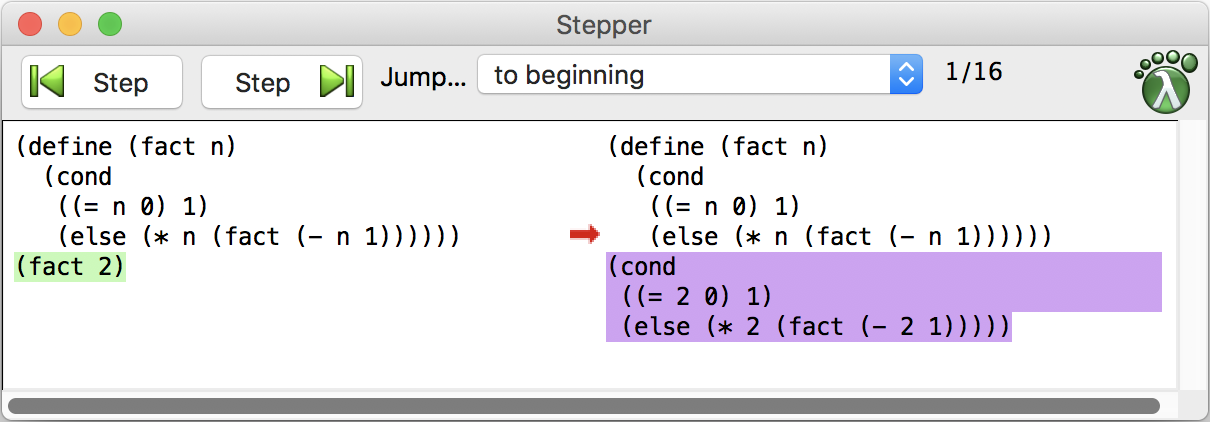
\includegraphics[width=13cm]{1/racket1.png}
  \end{center}
  \caption{DrRacket のステッパ}
  \label{figure:racket1}
\end{figure}

\begin{figure}
  \begin{center}
    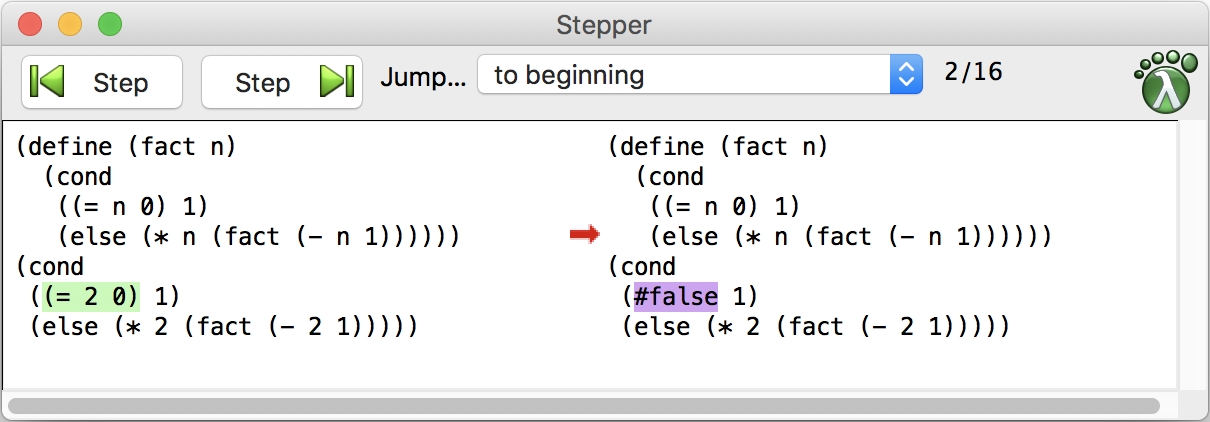
\includegraphics[width=13cm]{1/racket2.png}
  \end{center}
  \caption{DrRacket のステッパを進めた様子}
  \label{figure:racket2}
\end{figure}

我々は、プログラミング初心者がデバッグをするのに最適な方法は、ステッパを使うことだと考える。ステッパは Racket 言語の統合開発環境 DrRacket において提供されているツール\cite{clements01}である。ユーザがエディタにプログラムを書いてステッパ起動ボタンを押すと、図\ref{figure:racket1}のようなウインドウが表示される。図\ref{figure:racket1}は、再帰関数を用いて2の階乗を計算するプログラムを入力してステッパを起動したときの様子である。ウインドウには左右にそれぞれプログラムが表示されている。左はユーザが入力したプログラムと同じものであり、このプログラムで最初に簡約される式 \texttt{(fact 2)} が緑色にハイライトされている。右側のプログラムでは、ハイライトされた部分以外は左側と同じプログラムが表示されており、左側では緑色だった式 \texttt{(fact 2)} がその簡約結果に置き換えられ、紫色でハイライトされている。

Step ボタンのうち右の実行を進めるボタンを押すと図\ref{figure:racket2}のような表示に切り替わる。最初(図\ref{figure:racket1})は右側にあったプログラムと同じプログラムが左に表示され、次に簡約される部分式 \texttt{(= 2 0)} が緑色にハイライトされており、右側には同様にその部分が簡約されて紫色になったプログラムが表示されている。当初 \texttt{(fact 2)} だった式がその値である \texttt{2} になるステップまで、ボタンを押すと次々に簡約が行われてプログラムが変形していく様子を視覚的に見ることができる。

このように、プログラムを実行したときに、実行結果の値だけでなく、
実行中にプログラムが代数的にどのように書き換えられていくかを見せるツールがステッパである。
ステッパの操作は基本的に「前のステップへ」「次のステップへ」のボタンを押すのみであり、
プログラミングや CUI での操作に慣れていない初心者でも使いやすい。

しかし、
DrRacket のステッパが受け付けるのは Racket 言語のうちの一部の構文で構成された教育用の言語であり、
例外処理などの制御オペレータがサポートされていない。
初心者にとって理解しにくい言語機能を含むプログラムを
ステップ実行できるようにするために、
本研究ではそういった複雑な言語機能に対応したステッパを実装する方法を示す。

我々は、ステッパの動作を以下の 3 つに分けて処理した。

\begin{enumerate}
\item 入力されたプログラムを構文解析して構文木を得る。
\item ステッパ関数に構文木を渡して、ステップを出力しながら入力プログラムを実行する。
\item 出力文字列をユーザの操作に従って1つずつ表示する。
\end{enumerate}

\begin{figure}
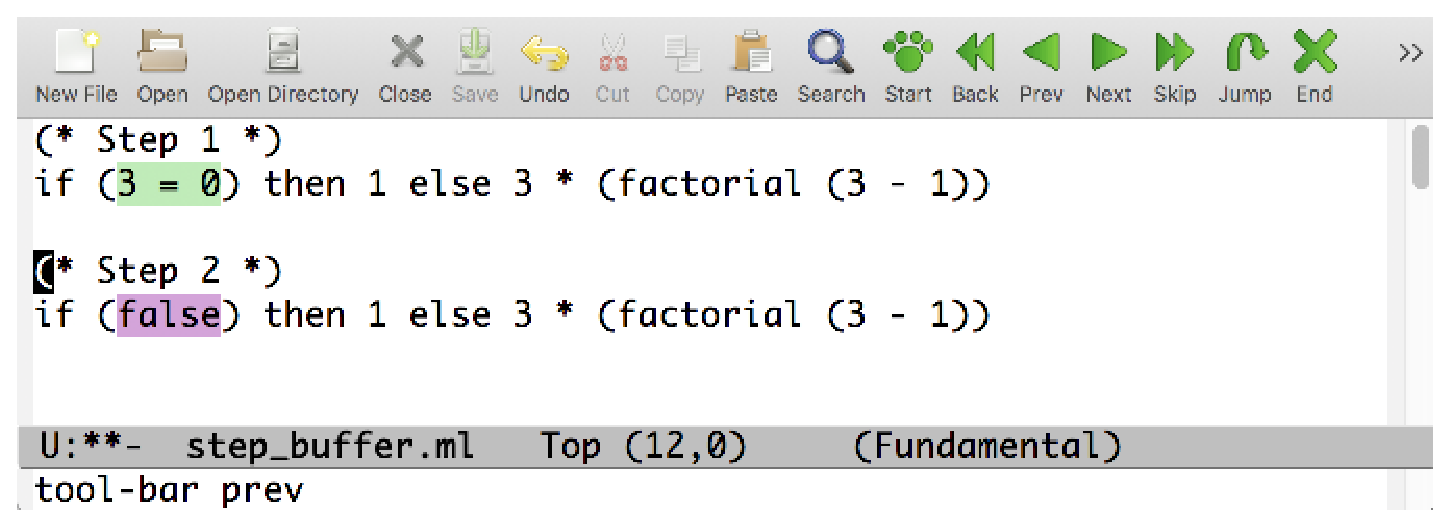
\includegraphics[width=13cm]{1/ocamlfac.eps}
\caption{本研究で実装した OCaml のステッパ}
\label{figure:ocamlfac}
\end{figure}

この中で最も重要なのは 2 つ目、すなわち
入力プログラムを表す構文木を受け取ってステップを表す文字列を出力する関数を作ることである。
それを実現する方法を本論文では 2 種類示している。
そして実装したステッパ (図 \ref{figure:ocamlfac}) を実際に大学の授業において使用し、
学生のプログラム実行ログやアンケートをもとに評価を行った。
その結果、上の 3 つの手順を順番に同期的に行うと
大規模なプログラムをステップ実行する際に 2 つ目の手順に長い時間がかかるため
表示を始めることができないという問題点が発覚した。
その解決のため、1 ステップの実行と表示処理を交互に行うので
ステップ実行処理の終了を待たずに利用できる「incremental なステッパ」を実装した。

\vspace{1cm}
以下に本論文の構成を示す。{\bf 第2章}では、関連研究について述べる。
{\bf 第3章}では、try-with を含む言語を対象にしたステッパの実装方法を説明する。
{\bf 第4章}では、第3章とは別の方法によって algebraic effects
を含む言語を対象にしたステッパの実装方法を説明する。
{\bf 第5章}では、1 ステップずつ実行する incremental なステッパの実装方法を紹介する。
{\bf 第6章}では、プログラミング学習におけるステッパの効果を考察する。
そして{\bf 第7章}で、結論を述べる。

\pagenumbering{arabic}

\chapter{関連研究}
\label{chapter:related}

\section{ステッパの実装}
\label{section:stepper__related}

ステッパはもともと Racket 言語の教育用に制限された構文に対して作られた。
これは Clements ら \cite{clements01} が設計したもので、
スタックに continuation mark と呼ばれるマークをつけることで
現在の評価文脈を再構成できるようにしている。
この Racket のステッパの対象構文には例外処理が含まれていない。

Whitington と Ridge \cite{EPTCS294.3} は
small-step のインタプリタを直接書くことで
OCaml に対するステッパを実装した。

PLT Redex \cite{felleisen09}は操作的意味論の形式化のための言語で、
文法と簡約規則を定義できるようになっており、DrRacket のステッパを継承している。
さらに、一画面の中に各ステップでのプログラムを配置し、
あるプログラムが1ステップ簡約されて別のプログラムになることを矢印で表したグラフを表示する。
これはより視覚的に簡約の様子を表すことができるほか、
各矢印にそのステップの簡約規則が添えられているのでよりステップを辿りやすい。
しかし、複数のステップのプログラムが同じ画面に表示されている上に
簡約が起こる部分式が強調されていないので、
長いプログラムをステップ実行すると見づらくなってしまう。

根岸ら\cite{NI2009}の関数型言語 Haskell のデバッガフロントエンドは、
一般的なデバッガの実行方法が通用しない遅延評価型言語の
グラフィカルなユーザインタフェースでのステップ実行を含むデバッガ操作を可能にした。
デバッガがブラウザ上で利用できるようになっており、
DrRacket や本研究のステッパと同様に各ステップでのプログラムを、
評価中の式をハイライトしながら表示する。
実行するファイルや、ブレイクポイントをどの関数に設定するか、
ステップ実行するか次のブレイクポイントまで実行するか、
などといった設定をブラウザ上のボタンなどをクリックすることで行うことができる。
デバッガのインタフェースでの本研究との違いは、
根岸ら\cite{NI2009}のデバッガではブレイクポイントをユーザが簡単に設定できるのに対して、
本研究ではブレイクポイントは自動的に全ての簡約基に設定され、
ユーザは詳細に実行のしかたを決められない代わりに「次のステップ」「前のステップ」
などのボタンを押すのみのより簡単な操作のみでステップ実行をすることができる。

\section{ステップ実行によるプログラミング学習}

Tunnel Wilson et al. \cite{tunnell18} は、
代数学的ステッパの出力のような内容を学生に手書きで書かせることによって、
学生がプログラムの実行のされかたをどのように理解しているか、
どのような構文のステップの書き下しができないかといった傾向を分析した。

\section{algebraic effects}
\label{section:algebraic effects__related}

本論文では algebraic effects に対する意味論を、
big-step で書かれた、ハンドラ内の実行について CPS になっているインタプリタで定義する。
Kammar ら \cite{10.1145/2500365.2500590} は small-step で意味論を与えた。
Hillerstr{\"o}m ら \cite{e6cb0c3222794e48bf38cf44e46fe4aa} は
CPS による意味論を与えたが、入力言語を A-正規形に制限しているのに加え、
継続がフレームのリストで与えられており、通常の CPS インタプリタにはなっていない。

上記以外の algebraic effects に関する研究としては、ハンドラの挙動が異
なる shallow ハンドラの研究 \cite{10.1007/978-3-030-02768-1_22} や
algebraic effects を含むプログラムに関する論理関係を
定義する研究 \cite{10.1145/3158096} などがあげられる。本論文で扱ってい
るハンドラは従来の deep ハンドラである。shallow ハンドラにも対応できると
考えているが、これは今後の課題である。


\chapter{try-with のステップ実行}
\label{chapter:try-with}

\section{はじめに}
\label{section:try-with__intro}

この章では、try-with 構文を含む言語を対象としたステッパ関数を
OCaml で実装する方法を示す。
OCaml 自体も try-with 構文で例外処理を行うので、
実際に我々が大学の授業において使っている OCaml ステッパは本章で説明する方法に基づいて実装されている。
ここでは簡単のため型無し $\lambda$ 計算と try-with 構文のみから成る言語を対象として説明する。

ステッパの実装は対象言語の通常のインタプリタ関数を拡張することによって行う。
この章ではまず \ref{section:try-with__interpreter} 節で言語とそのインタプリタを定義し、
\ref{section:try-with__stepper} 節でインタプリタを拡張してステッパを実装する。


 \section{対象言語とインタプリタの定義}
\label{section:try-with__interpreter}

\begin{figure}
\begin{spacing}{0.8}
\begin{verbatim}
type e_t = Var of string               (* x *)
         | Fun of string * e_t         (* fun x -> e *)
         | App of e_t * e_t            (* e e *)
         | Try of e_t * string * e_t   (* try e with x -> e *)
         | Raise of e_t                (* raise e *)
\end{verbatim}
\end{spacing}
\caption{対象言語の定義}
\label{figure:typee}
\end{figure}

\begin{figure}
\begin{spacing}{0.8}
\begin{verbatim}
(* 入力プログラムの例外の値を引数に持つ例外 *)
exception Error of e_t

(* 式を実行する *)
(* eval : e_t -> e_t *)
let rec eval expr = match expr with
  | Var (x) -> failwith ("unbound variable: " ^ x)  (* ここには来ない *)
  | Fun (x, e) -> Fun (x, e)
  | App (e1, e2) ->
    begin
      let v2 = eval e2 in
      let v1 = eval e1 in
      match v1 with
        | Fun (x, e) ->
          let e' = subst e x v2 in   (* e[v2/x] *)
          let v = eval e' in
          v
        | _ -> failwith "not a function"
    end
  | Try (e1, x, e2) ->
    begin
      try
        let v1 = eval e1 in
        v1
      with Error (v) ->
        let e2' = subst e2 x v in   (* e2[v/x] *)
        eval e2'
    end
  | Raise (e) ->
    let v = eval e in
    raise (Error (v))

(* 実行を開始する *)
(* start : e_t -> e_t *)
let start e =
  try
    eval e
  with
    Error v -> Raise v
\end{verbatim}
\end{spacing}
\caption{big-step インタプリタ}
\label{figure:interpreter}
\end{figure}


%In Figures \ref{figure:typee} and \ref{figure:interpreter},
%we define the object language as well as a big-step interpreter.
%The \texttt{eval} function evaluates a given expression following OCaml's call-by-value, right-to-left strategy.
型無し$\lambda$計算と try-with から成る言語の OCaml による定義を
図 \ref{figure:typee} に示す。
そしてこの言語に対する代入ベースで call-by-value かつ right-to-left
のインタプリタは図 \ref{figure:interpreter} のように定義できる。

%For instance, when given an application \texttt{e1 e2},
%it first evaluates the argument \texttt{e2}, then evaluates the function \texttt{e1}.
%Once the application has been turned into a redex, we perform $\beta$-reduction, and evaluate the post-reduction expression.
例えば関数適用 \texttt{e1 e2} を実行するときには、
まず引数部分 \texttt{e2} を実行して、次に関数部分 \texttt{e1} を実行する。
両方が値になったら $\beta$ 簡約を行い、簡約後の式を実行する。
%Note that, when the top-level expression is an executable, closed program, the input of the \texttt{eval} function cannot be a variable.  The reason is that we never touch a function's body before it receives an argument, and that $\beta$-reduction replaces lambda-bound variables with values.
引数 \texttt{expr} が変数 \texttt{Var} だった場合はエラー終了するように書かれているが、
これは入力されたプログラム全体が実行可能な閉じた式だった場合に
関数 \texttt{eval} の引数に変数がくることはありえないからである。
なぜありえないかというと、関数の本体の実行は必ず、引数を受け取って仮引数を実引数に置き換えた後に行うからである。

%Object-level exception handling is performed by the meta-level \texttt{try} and \texttt{raise} constructs.
入力プログラムの例外処理は、インタプリタで実際に(OCaml の機能の) \texttt{try} と \texttt{raise} を使って実行する。
%Specifically, when evaluating \texttt{raise e},
%we first evaluate \texttt{e} to some value \texttt{v},
%and then raise a meta-level (OCaml) exception \texttt{Error v}.
具体的には、式 \texttt{raise e} を実行する場合、
まず \texttt{e} を実行してその値 \texttt{v} を得る。
そしてメタレベルの (OCaml の) 例外 \texttt{Error v} を起こす。

%If an exception \texttt{Error v} was raised
%during evaluation of \texttt{e1} in \texttt{try e1 with x -> e2},
%the \texttt{eval} function ignores the rest of the computation in \texttt{e1},
%and evaluates \texttt{e2} with \texttt{v} substituted for \texttt{x}.
式 \texttt{try e1 with x -> e2} の \texttt{e1} を実行している間に
例外 \texttt{Error v} が発生した場合は、
関数 \texttt{eval} は \texttt{e1} の中の残りの計算を無視して、
\texttt{e2} の中の変数 \texttt{x} に値 \texttt{v} を代入した
式 \texttt{e2[v/x]} の実行に移る。
% This is exactly how OCaml's try-with construct works.
このように、OCaml の try-with 構文を利用して OCaml の try-with 構文と同じような動作を実現することができる。
%For convenience, we will hereafter call \texttt{e1} a \emph{tryee};
%the intention is that \texttt{e1} is
%the expression being ``tried'' by the handler.
try 節の式のことを、プログラム内では \texttt{tryee} という変数名で表していることがある。
これは、 try ハンドラによって「try されている」ということを意図している。

%The main function \texttt{start} calls \texttt{eval}
%in an exception handling context.
メイン関数である \texttt{start} が \texttt{eval} を呼び出すとき、
その呼び出しは try-with で囲まれている。
%From the construction,
%we can see that any expression that has a \texttt{raise e}
%with no matching \texttt{try} clause will be evaluated to \texttt{raise v}.
\texttt{Error v -> raise v} とあるように、
対応する \texttt{try} 節が無い \texttt{raise e} の実行結果は、
\texttt{e} の実行結果を \texttt{v} として \texttt{raise v} とする。
%For example, \texttt{2 + 3 + (raise 4) + 5} evaluates to \texttt{raise 4}.
例えば、 \texttt{2 + 3 + (raise 4) + 5} の実行結果は \texttt{raise 4} である。


\section{ステッパの実装}
\label{section:try-with__stepper}

% As stated in Section \ref{sec:intro},
% a stepper must display the whole program at each reduction step.
ステッパは各簡約ステップでのプログラムの全体を表示する必要がある。
% Consider the simple arithmetic expression \texttt{(1 + 2 * 3) + 4}.
% When step-executing this expression,
% we want to see the following reduction sequence:
例えば単純な算術式 \texttt{(1 + 2 * 3) + 4} をステップ実行するとき、
我々が期待するステップ列は以下である。
\[
\begin{array}{cl}
            & \mathtt{(1 + 2 * 3) + 4} \\
\rightarrow & \mathtt{(1 + 6) + 4} \\
\rightarrow & \mathtt{7 + 4} \\
\rightarrow & \mathtt{11}
\end{array}
\]

% The interpreter in Figure \ref{figure:interpreter}, however,
% does not immediately give us these steps.
しかし、図\ref{figure:interpreter} のプログラムに出力機能を加えても、
直ちにこのようなステップ出力は得られない。
% Suppose the \texttt{eval} function is evaluating
% the subexpression \texttt{2 * 3}.
関数 \texttt{eval} が部分式 \texttt{2 * 3} を実行している時のことを考えてみよう。
% We can display this subexpression using a printing function,
% but we do not have enough information to reconstruct the whole program.
式を出力する関数を用意すれば実行中の部分式 \texttt{2 * 3} は表示できるが、
プログラム全体を再構成するには情報が足りていない。
% What is missing here is the \emph{context} surrounding \texttt{2 * 3},
% namely \texttt{(1 + [.])\ + 4}
% (where \texttt{[.]} denotes the hole of the context).
ここで欠けているのは \texttt{2 * 3} を囲んでいる \emph{コンテキスト} すなわち
\texttt{(1 + [.])\ + 4} である。
(コンテキストの穴を \texttt{[.]} と表記する。)
% Hence, to implement a stepper,
% we need to keep track of every evaluation context we have traversed.  
したがって、ステッパを実装するためには、
それまでの評価文脈を追い続ける必要がある。

% In Figure \ref{figure:simpleplug},
% we define context frames as algebraic data of type \texttt{frame\_t}.
図 \ref{figure:simpleplug} で、 \texttt{frame\_t} 型の代数的データとしてコンテキストフレームを定義している。
% Each frame represents evaluation of some subexpression:
各フレームがなんらかの部分式の実行を表しており、
% \eg, \texttt{CAppR (e1)} tells us that we are evaluating
% the argument part of an application, whose function part is \texttt{e1}.
例えば \texttt{CAppR (e1)} は、関数部分が \texttt{e1} である関数適用の引数部分を
実行していることを表す。
% Evaluation contexts are defined as lists of these frames
% (spoiler alert: this does not work for exceptions).
評価文脈はこのフレームのリストで定義される。
% We then define the \texttt{plug} function,
% which reconstructs a program by wrapping the expression
% \texttt{expr} with context frames in \texttt{ctxt}. 
また■■、式 \texttt{expr} をコンテキストフレーム列 \texttt{ctxt} で囲んで
プログラムを再構成する関数 \texttt{plug} も定義する。

\begin{figure}
\begin{spacing}{0.8}
\begin{verbatim}
(* コンテキストフレーム *)
type frame_t = 
             | CAppR of e_t           (* e [.] *)
             | CAppL of e_t           (* [.] v  *)
             | CTry of string * e_t   (* try [.] with x -> e *)
             | CRaise                 (* raise [.] *)

(* コンテキスト *)
type c_t = frame_t list

(* 式全体を再構成する *)
(* plug : e_t -> c_t -> e_t *)
let rec plug expr ctxt = match ctxt with
  | [] -> expr
  | CAppR (e1) :: rest -> plug (App (e1, expr)) rest
  | CAppL (e2) :: rest -> plug (App (expr, e2)) rest
  | CTry (x, e2) :: rest -> plug (Try (expr, x, e2)) rest
  | CRaise :: rest -> plug (Raise expr) rest
\end{verbatim}
\end{spacing}
%\caption{Contexts and reconstruction function; first attempt}
\caption{コンテキストと再構成関数 (試作版)}
\label{figure:simpleplug}
\end{figure}

% Now, if we let the evaluation function receive
% an additional argument representing the context,
% we should be able to display all the steps of
% the arithmetic expression \texttt{(1 + 2 * 3) + 4}.
これで■■、関数 \texttt{eval} がコンテキストを表す追加の引数を受け取るようにすれば、
\texttt{(1 + 2 * 3) + 4} のような式のステップ表示ができるようになるはずである。
% For instance, when evaluating the subexpression \texttt{2 * 3},
% the extra argument will be a two-element list
% \texttt{[(1 + [.]);\ ([.]\ + 4)]},
% and we can obtain the whole program using the \texttt{plug} function.
例えば、部分式 \texttt{2 * 3} を実行している時、その新しい引数の値は
\texttt{[(1 + [.]);\ ([.]\ + 4)]} であり、
これを関数 \texttt{plug} に渡せばプログラム全体を得ることができる。

% The resulting stepper is essentially the CK abstract machine
% \cite{FF1986}, where the expression is the control string and the
% evaluation context is the continuation.
最終的に得られるステッパ■■は、式を control string■■、評価文脈を継続とみなすと、本質的にCK 機械 \cite{FF1986} であるといえる。
% Substitution is used to implement $\beta$-reduction.
% 代入は $\beta$ 簡約の実装のために用いられている■■。
% We did not implement the abstract machine directly but augmented a
% big-step interpreter, because we want to keep the correspondence between
% big-step execution and small-step execution.
big-step インタプリタと small-step インタプリタの実行の対応を維持するため、
抽象機械を直接実装するのではなく big-step インタプリタの拡張によって実装した。
% 抽象マシンを直接実装するのではなく、
% 大きなステップの実行と小さなステップの実行との対応を維持したいため、
% 大きなステップのインタープリターを追加しました。
% It enables us to skip evaluation of user-specified function application,
% as we elaborate in Section~\ref{sec:imp:ocaml}.
big-step インタプリタを基にすることで、ユーザが指定した関数適用をスキップすることができる
(\ref{section:experiment__language} 節で触れる)。

% Unfortunately,
% this na\"ive implementation does not work
% in the presence of exception handlers.
しかし、この実装は例外処理について正しく機能しない。
% Consider \texttt{try (2 + 3 * (raise 4) + 5) with x -> x}.
例えば、 \texttt{try (2 + 3 * (raise 4) + 5) with x -> x} について考える。
% When step-executing this expression, we expect to see the following steps:
この式をステップ実行する時、我々が期待するステップは以下である。

\vspace{0.2cm}

\noindent \texttt{(* Step 0 *) try (\colorbox{lightgreen}{2 + (3 * (raise 4)) + 5}) with x -> x\\
  (* Step 1 *) try (\colorbox{purple}{raise 4}) with x -> x\\
  (* Step 1 *) \colorbox{lightgreen}{try (raise 4) with x -> x}\\
  (* Step 2 *) \colorbox{purple}{4}\\
}

\vspace{0.2cm}

% \noindent The first reduction happens when the input
% to the stepping interpreter is \texttt{raise 4}.
\noindent 最初の簡約はステッパ関数に \texttt{raise 4} が渡されたときに起こる。
% However, observe that the highlighted redex is a bigger expression
% \texttt{(2 + 3 * (raise 4) + 5)},
% because reduction of a \texttt{raise} construct discards
% the context \emph{within} the tryee.
しかし、最初のステップでハイライトされている式はそれよりも大きい式
\texttt{(2 + 3 * (raise 4) + 5)} である。
これは \texttt{raise 4} の実行で例外を起こす際に、この式の外側にある、tryee の内部のコンテキストを捨てるからである。
% Since context frames are collected in a single list,
% the second argument at this point will be
% \texttt{[(3 * [.]); (2 + [.]);\ ([.]\ + 5);\ (try [.]\ with x -> x)]},
% \ie, it contains the context \emph{outside} the tryee.
コンレキストフレームは 1 つのリストに入っているので、この時点での関数 \texttt{eval} の第2引数は
\texttt{[(3 * [.]); (2 + [.]);\ ([.]\ + 5);\ (try [.]\ with x -> x)]} であり、
すなわち tryee の外側のコンテキストを含んでいる。
% This suggests that, when dealing with exception handlers,
% we have to distinguish between contexts inside and outside a tryee.
例外処理を扱う場合には、tryee の内側と外側のコンテキストを区別する必要があるということである。
\footnote{
% The destination is not necessary,
% if we want to support only exception handling.
例外処理をサポートするだけならばこの■■必要はない。
% We could simply search for the enclosing handler in the evaluation
% context.
コンテキストフレームのリストを単純に検索すれば最も内側のハンドラを見つけることができるからである。
% However, it requires a linear search through the evaluation context.
しかし、それには評価文脈を線形探索する必要がある。
% Furthermore, distinction is necessary if we want to implement
% more general control operators,
% such as shift and reset \cite{DF1990}.
さらに、shift/reset のようなより一般的な制御オペレータ■■を実装する場合には
この区別が必要になる。
}

\begin{figure}
\begin{spacing}{0.8}
\begin{verbatim}
(* コンテキストフレーム *)
type frame_t = 
             | CAppR of e_t          (* e [.] *)
             | CAppL of e_t          (* [.] v *)
             | CRaise                (* raise [.] *)

(* try フレーム *)
type ctry_t = 
            | CHole                        (* [.] *)
            | CTry of string * e_t * c_t   (* try [.] with x -> e *)

(* コンテキスト *)
and c_t = frame_t list * ctry_t

(* tryee を再構成する *)
(* plug_in_try : e_t -> frame_t list -> e_t *)
let rec plug_in_try expr ctxt = match ctxt with
  | [] -> expr
  | first :: rest -> match first with
    | CAppR (e1) -> plug_in_try (App (e1, expr)) rest
    | CAppL (e2) -> plug_in_try (App (expr, e2)) rest
    | CRaise -> plug_in_try (Raise (expr)) rest

(* プログラム全体を再構成する *)
(* plug : e_t -> c_t -> e_t *)
let rec plug expr (clist, tries) =
  let tryee = plug_in_try expr clist in
  match tries with
  | CHole -> tryee
  | CTry (x, e2, outer) -> plug (Try (tryee, x, e2)) outer
\end{verbatim}
\end{spacing}
%   \caption{Contexts and reconstruction function; final version}
  \caption{コンテキストと再構成関数 (最終版)}
  \label{figure:typec}
\end{figure}

% In Figure \ref{figure:typec},
% we present a refined definition of evaluation contexts.
図 \ref{figure:typec} に、改良したコンテキスト定義を示す。
% We see a new definition of context frames \texttt{frame\_t},
% where \texttt{CTry} is missing.
新しい \texttt{frame\_t} 型の定義は、 \texttt{CTry} を含まないようになっている。
% When evaluating a program that uses try-with constructs,
% these frames are used to build a delimited context within a tryee.
\texttt{frame\_t} 型のフレームは、try-with 構文を使うプログラムを実行において
tryee の内部に限定されたコンテキストを表すために使う。
% We next find a separate datatype \texttt{ctry\_t},
% which can be understood as meta contexts.
次に、別の型 \texttt{ctry\_t} が定義されており、これはメタコンテキストを表す型である。
% Then we define evaluation contexts as pairs of delimited and meta contexts.
そしてコンテキストは tryee 内部に限定されたコンテキストとメタコンテキストの 2 つ組として定義される。
% As an example, when evaluating \texttt{raise 4} in the following expression:
例として、以下のプログラムの中の \texttt{raise 4} を実行しているとき、

\begin{verbatim}
0 + (try 1 + 2 * (try (3 + raise 4) - 5 with x -> x + 6) with y -> y)
\end{verbatim}
% \noindent the current context looks like:
\noindent 現在のコンテキストは以下のようになっている。
\begin{verbatim}
([(3 + [.]); ([.] - 5)],
  CTry ("x", x + 6,
    ([2 * [.]; 1 + [.]],
      CTry ("y", y,
        ([0 + [.]], CHole)))))
\end{verbatim}

% The refined contexts allow us to first reconstruct the expression up to
% the tryee using the \texttt{frame\_t} contexts,
% and then build up the whole program using the \texttt{ctry\_t} contexts.
このようにコンテキスト定義を改良すると、
まず \texttt{frame\_t} 型のコンテキストを使って tryee 式を再構成し、
その後 \texttt{ctry\_t} 型のコンテキストを使ってプログラム全体を作ることができる。
% In our particular example, the stepper reconstructs \texttt{(3 + raise 4) - 5},
% highlights it, and reconstructs the whole program.
上の例でいうと、ステッパはまず \texttt{(3 + raise 4) - 5} を再構成して
ハイライトしてから、プログラム全体を再構成している。

% To give the reader a better idea how context frames are accumulated,
% let us demonstrate the evaluation of an expression involving exception handling:
コンテキストフレームが蓄積されていく様子を具体的に紹介するため、
例外処理を含んだ式の実行で関数 \texttt{eval} がどのような順で再帰呼び出しされるかを以下に示す。

\begin{verbatim}
eval (2 * (try 3 + (raise 4) - 5 with x -> x + 6)) ([], CHole)
eval (try 3 + (raise 4) - 5 with x -> x + 6) ([2 * [.]], CHole)
eval (3 + (raise 4) - 5) ([], CTry ("x", x + 6, ([2 * [.]], CHole)))
eval 5 ([3 + (raise 4) - [.]], CTry ("x", x + 6, ([2 * [.]], CHole)))
eval (3 + (raise 4)) ([[.] - 5], CTry ("x", x + 6, ([2 * [.]], CHole)))
eval (raise 4) ([3 + [.]; [.] - 5], CTry ("x", x + 6, ([2 * [.]], CHole)))
eval 4 ([raise [.]; 3 + [.]; [.] - 5], CTry ("x", x + 6, ([2 * [.]], CHole)))
eval (4 + 6) ([2 * [.]], CHole)
\end{verbatim}

% \noindent Observe that we discard the context within the tryee,
% namely \texttt{3 + (raise [.])\ - 5}, at the last step.
\noindent 最後のステップにおいて、tryee の内部のコンテキスト
すなわち \texttt{3 + (raise [.])\ - 5} が捨てられている。

% Now we present our stepping interpreter in Figure \ref{figure:stepper}.
以上を踏まえ、ステッパ関数を図 \ref{figure:stepper} および図 \ref{figure:try-with__memo} に示す。
% The function extends the big-step interpreter in two ways
% (as shaded in the figure):
この関数は通常の big-step インタプリタを以下の 2 点において拡張したものである (図中の灰色の部分)。
% (i) it receives an argument representing the evaluation context;
(i) コンテキストを表す引数を受け取るようにする。
% and (ii) it outputs the current program every time reduction takes place.
(ii) 簡約が行われる全ての箇所で簡約前後のプログラムをそれぞれ出力する。

\begin{figure}
%(* add a non-try frame *)
%(* add : c_t -> frame_t -> c_t *)
%let rec add (list, outer) ctxt = (ctxt :: list, outer)
%
%(* add a try frame *)
%(* add_try : c_t -> string -> e_t -> c_t *)
%let rec add_try ctxt var expr = ([], CTry (var, expr, ctxt))  
\begin{spacing}{0.8}
\begin{alltt}
(* ステッパ関数 *)
(* eval : e_t -> c_t -> e_t *)
let rec eval expr \colorbox{lightgray}{ctxt} = match expr with    (* コンテキストのための引数を増やす *)
  | Var (x) -> failwith ("unbound variable: " ^ x)
  | Lam (x, e) -> Lam (x, e)
  | App (e1, e2) ->
    begin
      let v2 = eval e2 \colorbox{lightgray}{(add ctxt (CAppR e1))} in     (* コンテキスト情報を足す *)
      let v1 = eval e1 \colorbox{lightgray}{(add ctxt (CAppL v2))} in     (* コンテキスト情報を足す *)
      match v1 with
      | Lam (x, e) ->
        let e' = subst e x v2 in
        \colorbox{lightgray}{memo (App (v1, v2)) e' ctxt;}                                (* 出力 *)
        let v = eval e' \colorbox{lightgray}{ctxt} in                     (* コンテキスト情報を足す *)
        v
      | _ -> failwith "not a function"
    end
  | Try (e1, x, e2) ->
    begin
      try
        let v1 = eval e1 \colorbox{lightgray}{(add_try ctxt x e2)} in     (* コンテキスト情報を足す *)
        \colorbox{lightgray}{memo (Try (v1, x, e2)) v1 ctxt;}                             (* 出力 *)
        v1
      with Error (v) ->
        let e2' = subst e2 x v in
        \colorbox{lightgray}{memo (Try (Raise v, x, e2)) e2' ctxt;}                       (* 出力 *)
        eval e2' \colorbox{lightgray}{ctxt}                               (* コンテキスト情報を足す *)
    end
  | Raise (e0) ->
    let v = eval e0 \colorbox{lightgray}{(add ctxt CRaise)} in            (* コンテキスト情報を足す *)
    \colorbox{lightgray}{begin match ctxt with                   }
\end{alltt}
\vspace{-27pt}
\begin{alltt}
    \colorbox{lightgray}{    | ([], _) -> ()                     }
\end{alltt}
\vspace{-27pt}
\begin{alltt}
    \colorbox{lightgray}{    | (clist, tries) ->                 }
\end{alltt}
\vspace{-27pt}
\begin{alltt}
    \colorbox{lightgray}{      memo (plug_in_try (Raise v) clist)}                        (* 出力 *)
\end{alltt}
\vspace{-27pt}
\begin{alltt}
    \colorbox{lightgray}{           (Raise v)                    }
\end{alltt}
\vspace{-27pt}
\begin{alltt}
    \colorbox{lightgray}{           ([], tries)                  }
\end{alltt}
\vspace{-27pt}
\begin{alltt}
    \colorbox{lightgray}{end;                                    }
    raise (Error (v))
\end{alltt}
\end{spacing}
% \caption{Stepping evaluator}
\caption{ステッパ関数}
\label{figure:stepper}
\end{figure}

\begin{figure}
\begin{spacing}{0.8}
\begin{alltt}
(* 簡約前の式と簡約後の式とコンテキストを受け取ってステップを出力する *)
(* memo : e_t -> e_t -> c_t -> unit *)
let memo expr1 expr2 ctxt =
  print_exp (plug (green expr1) ctxt);
  print_exp (plug (purple expr2) ctxt)

(* ステップ実行を始める *)
(* start : e_t -> e_t *)
let start e =
  try
    eval e \colorbox{lightgray}{([], CHole)}    (* 空のコンテキスト *)
  with
    Error (v) -> (Raise v)
\end{alltt}
\end{spacing}
% \caption{\texttt{memo} and main functions}
\caption{関数 \texttt{memo} とメイン関数}
\label{figure:try-with__memo}
\end{figure}

% Let us observe the application case.
まず関数適用 \texttt{e1 e2} のケースの動作を見ると、以下のようになっている。
% As in the big-step interpreter,
% we first evaluate \texttt{e2}, and then \texttt{e1}.
通常のインタプリタと同じように、最初に \texttt{e2} を実行してその後に \texttt{e1} を実行する。
% When \texttt{e1} has reduced to a function,
% we know that the application is a $\beta$-redex.
\texttt{e1} の実行結果が関数であれば、関数適用式は $\beta$ 簡約基になっている。
% In the standard interpreter,
% what we do is to perform the substitution \texttt{subst e x v2}
% and then evaluate the result.
通常のインタプリタでは、そこで代入 \texttt{subst e x v2} をしてその結果を実行する。
% In the stepper, on the other hand,
% we have an additional function call to the \texttt{memo} function
% defined in Figure \ref{figure:memo}.
それに対しステッパでは、
図 \ref{figure:try-with__memo} で定義された関数 \texttt{memo} の呼び出しが追加されている。
% This function receives three arguments:
% the redex we have just found, its reduct, and the current evaluation context.
この関数は 3 つの引数を受け取る。
見つかった簡約基と、その簡約結果と、現時点のコンテキストである。
% When given these arguments,
% the \texttt{memo} function reconstructs and prints the pre- and post-reduction programs,
% using the \texttt{plug} and \texttt{print\_exp} functions
関数 \texttt{memo} はこれらの引数を受け取ったら、
関数 \texttt{plug} と \texttt{print\_exp} を使って簡約前と後のプログラムをそれぞれ再構成して出力する。
\footnote{
    % In the actual implementation,
    % we annotate redexes and reducts using OCaml's \emph{attributes}.
    実際の実装においては、簡約基と簡約後の式の範囲を表す情報をつけるのに
    OCaml の \emph{attributes} という機能を利用している。
    % Here, we write \texttt{green expr1} to mean \texttt{expr1[@stepper.redex]},
    % and similarly for \texttt{purple}.
    ここでは \texttt{green expr1} は \texttt{expr1[@stepper.redex]} と出力される式を表し、
    \texttt{purple} についても同様である。
    % When displaying the steps,
    % the Emacs Lisp program uses the attributes information
    % to appropriately highlight expressions.
    ステップを表示する際に、 Emacs Lisp のプログラムがその情報から
    適切に式をハイライトする。
    }
    % .  After printing the programs, we continue evaluation as usual.
    。プログラムを出力したら、普通の実行を再開する。

% In the \texttt{eval} function, we find three more occurrences of \texttt{memo},
% representing the following reduction rules:
関数 \texttt{eval} では、これ以外にあと 3 箇所で関数 \texttt{memo} が呼び出されている。
それらはそれぞれ以下の簡約規則を表している。

\begin{itemize}
  \item \texttt{try v with x -> e} $\leadsto$ \texttt{v}
  \item \texttt{try raise v with x -> e2} $\leadsto$ \texttt{subst e2 x v}
  \item \texttt{...\ (raise v) ...} $\leadsto$ \texttt{raise v}
\end{itemize}

% \noindent Note that,
% although the second reduction always happens right after the third one,
% we keep them as separate rules.
\noindent 2 つ目の簡約は必ず 3 つ目の簡約の直後に起こるが、
それにもかかわらずこれらを別の規則として扱っていることに注目してほしい。
% The reason is that we need the latter to reduce
% a raise construct with no matching try clause:
その理由は、例えば \texttt{3 + (raise 4) - 5} $\leadsto$ \texttt{raise 4} のように
対応する try 節が無い \texttt{raise} 式の簡約に 3 つ目の規則が必要だからである。
% \eg, \texttt{3 + (raise 4) - 5} $\leadsto$ \texttt{raise 4}.
% Separating the two reductions also has an educational benefit:
% it clearly tells us that exception handling consists of two tasks:
% discarding the context and substituting the value.
また、これらの規則を別にしておくのは教育上の意義もある。
それは、例外処理が「コンテキストを捨てること」と「例外の値を代入すること」
の 2 つの動作で成り立っていることが明確にステップに表れることである。

%% By observing what we pass to the \texttt{memo} function, we can see the reduction rules of the object language.  In the definition of \texttt{eval}, we have four occurrences \texttt{memo}, representing the following reduction rules:

%% \begin{enumerate}
%% \item
%%   \texttt{(fun x -> e) v} $\leadsto$ \texttt{subst e x v}
%%   \begin{itemize}
%%   \item \texttt{\colorbox{lightgreen}{f 4} + 100} (where \texttt{f = fun x -> x * 2 + 1}) reduces to \texttt{(\colorbox{purple}{4 * 2 + 1}) + 100}.
%%   \end{itemize}
%% \item
%%   \texttt{try v with x -> e} $\leadsto$ \texttt{v}
%%   \begin{itemize}
%%   \item \texttt{\colorbox{lightgreen}{try 2 with x -> x * x}} reduces to \texttt{\colorbox{purple}{2}}.
%%   \end{itemize}
%% \item
%%   \texttt{try raise v with x -> e2} $\leadsto$ \texttt{subst e2 x v}
%%   \begin{itemize}
%%   \item \texttt{\colorbox{lightgreen}{try raise 4 with x -> x * x}} reduces to \texttt{\colorbox{purple}{4 * 4}}.
%%   \end{itemize}
%% \item
%%   \texttt{try ...\ (raise v) ...\ with x -> e2} $\leadsto$ \texttt{try raise v with x -> e2}
%%   \begin{itemize}
%%   \item \texttt{try \colorbox{lightgreen}{1 + 2 + (raise 4) - 5} with x -> x * x} reduces to \texttt{try \colorbox{purple}{raise 4} with x -> x * x}.
%%   \end{itemize}
%% \end{enumerate}


\section{実際の OCaml ステッパ}
\label{section:ocaml stepper}

我々が実装した OCaml ステッパは、
\ref{section:try-with__stepper} 節で示した try-with と型無し $\lambda$ 計算に対するステッパと比べて
以下のような特徴がある。

\begin{itemize}
\item 型エラー等を想定しない。
\item 授業「関数型言語」で使用する構文のほぼ全てに対応している。
\item 関数適用が $\beta$ 簡約されるステップからその式が値になるステップまで飛ばす機能がある。
\end{itemize}

この節ではそれぞれについて述べる。

\subsection{型エラーについて}
\label{subsection:stepper__type}

OCaml ステッパでは、
まず入力プログラムを OCaml のパーザを利用して構文木にし、型チェックをする。
未定義変数エラーを含むシンタックスエラーや型エラーになった場合は
ステッパ本体のプログラムを起動せず、OCaml が示すエラーメッセージを表示する。
よって、コンパイルエラーがあるプログラムの構文木がステッパ関数に渡されることは無いという
仮定の上で実装されている。
ゼロ除算等の実行時エラーに関しては OCaml では例外の発生として処理されるので、
そのようにステップ実行処理を続行する。
ただし、例外が捕捉されないままその文の実行が終わってしまった場合はそこでステップ実行を終了する。

\subsection{対象構文}
\label{subsection:stepper__syntax}
% In Figure \ref{figure:ocamlstep},
% we show a reduction sequence produced by the actual stepping evaluator.
% 我々が実装した OCaml ステッパが出力するステップ列の例を図 \ref{figure:ocamlstep} に示す。
% The evaluator supports the following syntactic constructs:
このステッパは以下の構文に対応している。

\begin{itemize}
% \item integers, floating point numbers, booleans, characters, strings
% \item lists, tuples, records
% \item user-defined datatypes
% \item conditionals, let-expressions, recursive functions, pattern-matching
% \item exception handling operators
% \item printing functions and sequential execution
% \item the List module, user-defined modules
% \item references, arrays
\item 整数、実数、真偽値、文字、文字列型
\item リスト、組、レコード
\item ユーザ定義型
\item 条件分岐、変数定義、再帰関数定義、パターンマッチ
\item List モジュール、ユーザ定義モジュール
\item 例外処理
\item 標準出力関数、逐次実行
\item 書き換え可能な変数、配列
\end{itemize}

標準出力や書き換え可能な変数を含むプログラムでは、
標準出力された文字列や変数に格納された値などの「状態」をインタプリタが保持する必要がある。
状態の情報はステッパプログラム内の書き換え可能なグローバル変数の中に格納することで実装した。

\begin{figure}
  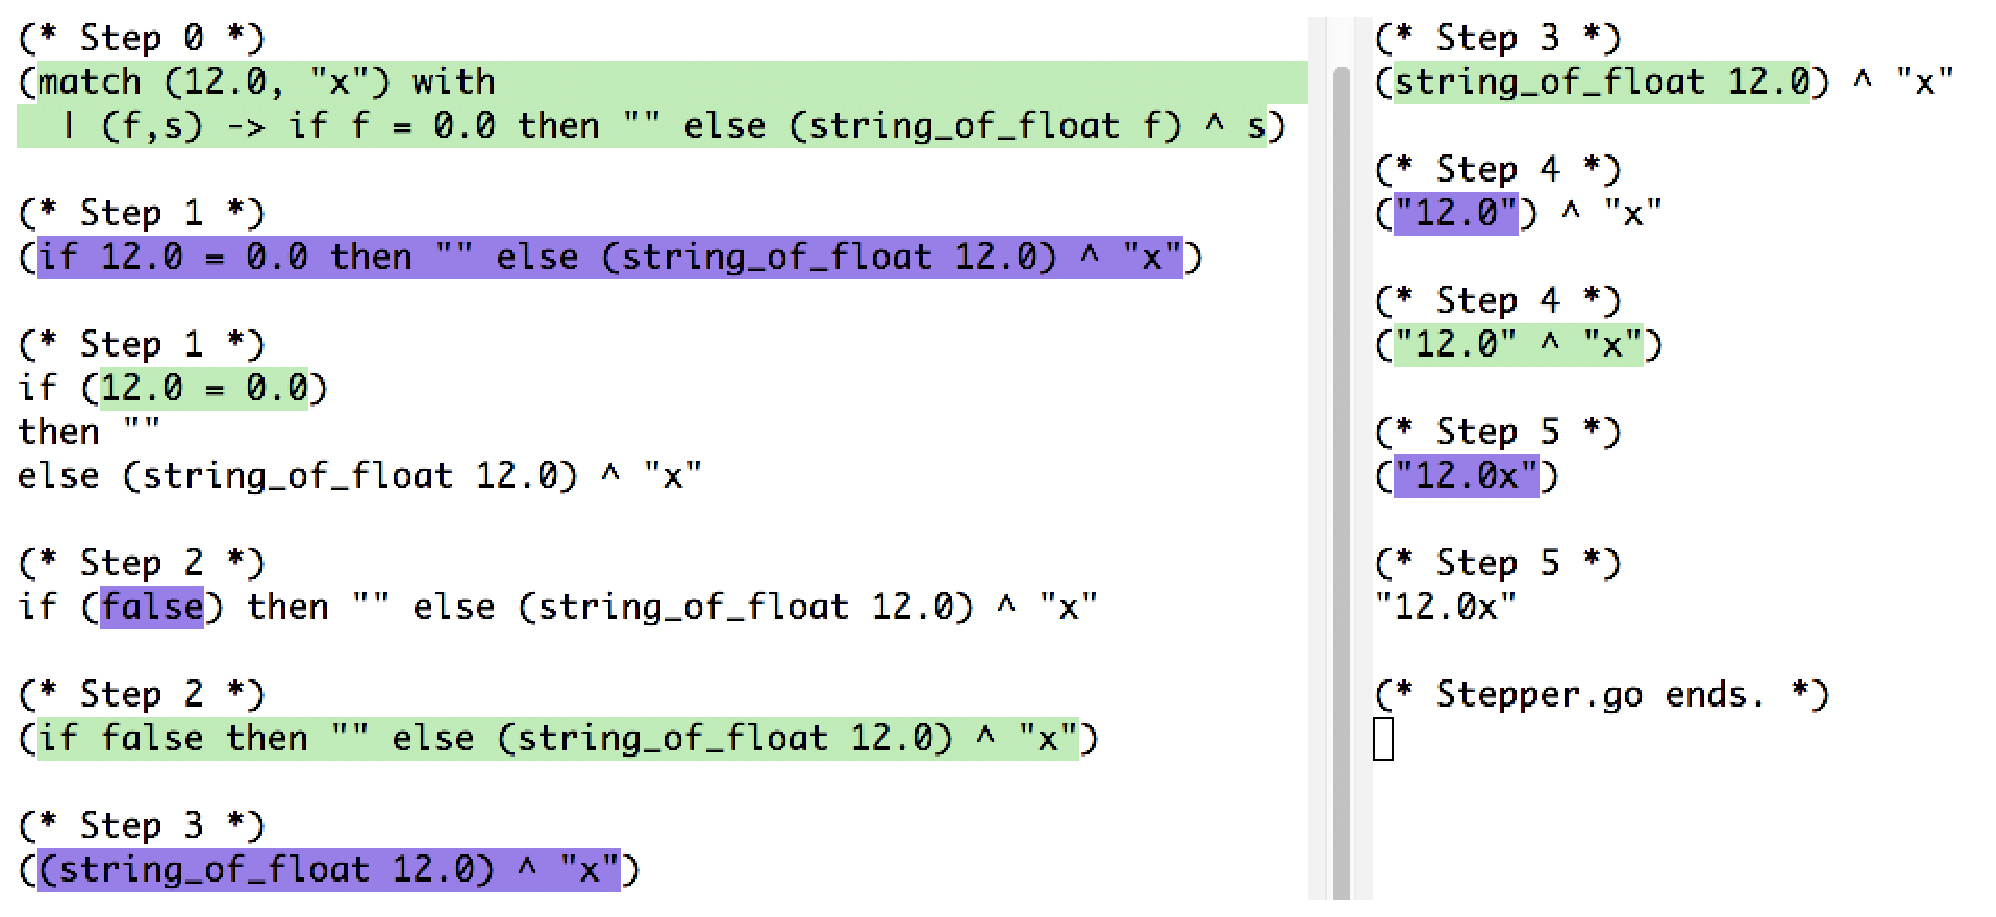
\includegraphics[width=14cm]{6/longexample.eps}
%   \caption{Evaluating programs using the actual stepper}
  \caption{実際のステッパでプログラムを実行する様子}
  \label{figure:ocamlstep}
\end{figure}

OCaml ステッパは他に授業で利用する一部の演算子などに対応している。
図 \ref{figure:ocamlstep} に実際のステップ列の例を示す。

% ref、配列を使うやつにする?

\subsection{関数適用のスキップ}
\label{subsection:skip}

\begin{figure}
  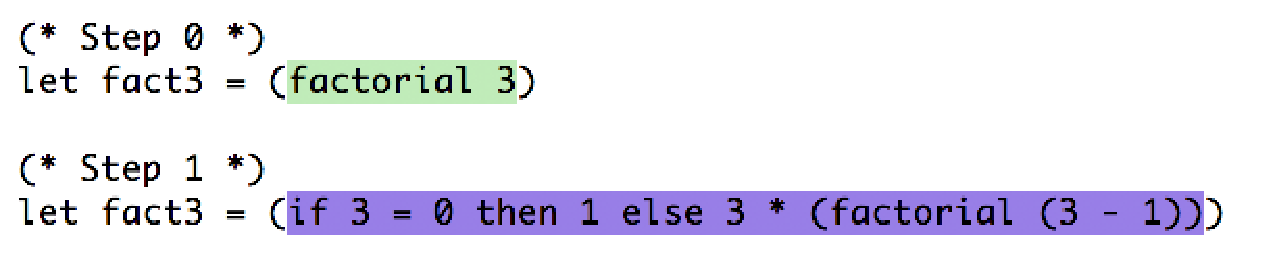
\includegraphics[width=10cm]{6/beforeskip.eps}
  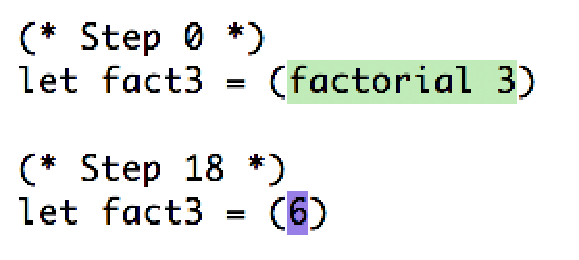
\includegraphics[width=4.3cm]{6/afterskip.eps}
%   \caption{Skipping evaluation of the factorial function}
  \caption{階乗関数をスキップする様子}
  \label{figure:factskip}
\end{figure}

% To allow the user to adjust granularity of steps,
% we provide an option for skipping
% the evaluation of the current function application.
プログラムのステップ数が多くなると、デバッグの目的でステップ実行をするときに
膨大な計算ステップを1つ1つ追って見るのは効率が悪く、
次第に実用に耐えるものではなくなってしまう。
そこで本研究では、「関数適用」を基準としてステップを飛ばす機能を追加した。

% Let us look at Figure \ref{figure:factskip},
% which shows skipping of the factorial function.
図 \ref{figure:factskip} に、階乗関数のスキップの様子を示す。
% By pressing the ``skip'' button,
% we can directly go from the program on the left to the one on the right,
% without seeing the intermediate steps that appear
% during the evaluation of the function's body.
左の状態で「skip」ボタンを押すと、関数の中身
\texttt{if 3 = 0 then 1 else 3 * (factorial (3 - 1))} が
\texttt{6} になるまでの実行ステップを見ることなく右の画面に移ることができる。
% This feature helps us focus on the steps we are interested in,
% allowing us to grasp the overall flow of the execution.
これによって見たいステップだけに注目することができ、実行の全体の流れを把握しやすくなる。

% The skipping feature requires some modifications to
% the \texttt{eval} function (Figure \ref{figure:skipapp}).
このスキップ機能は、
\ref{chapter:try-with} 章で try-with に対応したステッパ関数
(図 \ref{figure:stepper}) の eval 関数を
図 \ref{figure:skipapp} のように変更することで実装できる。
% The idea is to sandwich the steps within an application between two strings:
本研究では、飛ばすステップ列を
% \texttt{(* Application n start *)} and \texttt{(* Application n end *)}.
\texttt{(* Application n start *)} と \texttt{(* Application n end *)}
という 2 つの文字列で挟む方法をとった。
% Here, \texttt{n} tells us at which step we have entered the application.
\texttt{n} は関数適用の実行が始まるステップの番号である。
あるステップで実行が始まる関数適用は必ず 1 つ以下なので、
このステップ番号によって関数適用を一意に特定することができる。
% These strings are printed using the \texttt{apply\US start} and
% \texttt{apply\US end} functions,
% and help the Emacs Lisp program to hide unnecessary steps.
関数 \texttt{apply\US start :\ unit -> int} が前者を出力する関数、
関数 \texttt{apply\US end :\ int -> unit} が後者を出力する関数である。
表示処理をする Emacs Lisp プログラムがこれらの文字列を検索し、
間のステップを隠す処理をする。
% We show an example output sequence in Figure \ref{figure:skipping}.
スキップ機能を追加したステッパ関数の出力は例えば図 \ref{figure:skipping} のようになる。

\begin{figure}
\begin{alltt}
let rec eval expr ctxt = match expr with
    ...
  | App (e1, e2) ->
    begin
      let v2 = eval e2 (add ctxt (CAppR e1)) in
      let v1 = eval e1 (add ctxt (CAppL v2)) in
      match v1 with
        | Lam (x, e) ->
          let e' = subst e x v2 in
          \colorbox{lightgray}{let apply_num = apply_start () in}               (* 開始マークを出力 *)
          memo (App (v1, v2)) e' ctxt;
          let v = eval e' ctxt in
          \colorbox{lightgray}{apply_end apply_num;}                            (* 終了マークを出力 *)
          v
        | _ -> failwith "not a function"
    end
  | ...
\end{alltt}
\caption{関数適用をスキップするためのステッパ関数}
\label{figure:skipapp}
\end{figure}

\begin{figure}
\texttt{(* Step 0 *) (f 4) + \colorbox{lightgreen}{10 * 100}\\
(* Step 1 *) (f 4) + \colorbox{purple}{1000}\\
(* Application 1 start *)\\
(* Step 1 *) \colorbox{lightgreen}{f 4} + 1000\\
(* Step 2 *) \colorbox{purple}{(4 * 2) - 1} + 1000\\
(* Step 2 *) \colorbox{lightgreen}{(4 * 2} - 1) + 1000\\
(* Step 3 *) \colorbox{purple}{(8} - 1) + 1000\\
(* Step 3 *) \colorbox{lightgreen}{8 - 1} + 1000\\
(* Step 4 *) \colorbox{purple}{7} + 1000\\
(* Application 1 end *)\\
(* Step 4 *) \colorbox{lightgreen}{7 + 1000}\\
(* Step 5 *) \colorbox{purple}{1007}}
\caption{関数適用をスキップするためのステッパ関数の出力}
\label{figure:skipping}
\end{figure}


\section{この章のまとめ}
\label{section:try-with__conclusion}

この章では、例外処理の構文 try-with に対応したステッパを、
インタプリタを拡張することによって実装する方法を示した。

まず、 try-with 構文に対する通常の big-step インタプリタは
実際の OCaml の try-with を用いて実装することができた。

ステッパへの拡張においては、各ステップでのプログラム全体を表示するために、
実行中の部分式のコンテキストの情報が必要である。
例外発生によって一度に捨てられる範囲のコンテキスト、
すなわち try 節の内側のコンテキストフレームをひとまとまりにして、
そのリストを要素に持つリストのような構造としてコンテキストを定義した。
それをインタプリタの再帰の構造にしたがって要素を足しながら引数に渡すようにすると
実行中の部分式のコンテキストの情報が得られるようになり、
プログラム全体が出力できるステッパが得られた。



\chapter{4}


\chapter{incremental なステッパの実装}
\label{chapter:incremental}

\section{ステッパの動作}

本章で説明する incremental なステッパは、表面上は \ref{chapter:try-with} 章のステッパと同じ動作をするが、
内部での処理方法および速さが大きく異なる。
本節では、既存のステッパと本章の incremental なステッパのそれぞれの動作について説明する。

いずれのステッパも、実行可能な1つのプログラムを対象としている。

\subsection{DrRacketのステッパ}
\label{ステッパの動作-DrRacketのステッパ}
DrRacket のステッパ\cite{clements01}は、ユーザが入力したプログラムを全ステップの情報を生成するプログラムへ変換し、それを実行してステップの情報を蓄えながら、ユーザの操作に従って1つのステップを表示する。実行開始に少し遅れて、表示のための処理を並列して行うことになる。

\subsection{incremental でない OCaml ステッパ}
\label{ステッパの動作-incrementalでないOCamlステッパ}

\ref{chapter:try-with} 章で実装した OCaml ステッパ (以下、incremental でない OCaml ステッパ) では、
では、インタプリタにステップ出力機能を足したものに入力プログラムを渡し、
全ステップの文字列を生成する。
プログラムを全て実行するかステップ数の上限に達すると実行を終了し、
最初のステップを表示し、
ユーザの操作に従って表示するステップを変える。

インタプリタは新しく我々が作った OCaml の関数であり、通常のインタプリタよりも実行速度が遅い。そこにさらに出力機能を足したインタプリタによるプログラム実行が終わるまで表示が始まらないため、実行に時間がかかるプログラムのステップ実行をするには長い時間待つ必要がある。

\subsection{提案するステッパ}
\label{ステッパの動作-提案するステッパ}

本章で提案するステッパは、インタプリタにステップ出力機能を足したものに入力プログラムを渡し、1ステップの簡約を計算したらただちにそのステップを出力し、続きの実行は行わずにプロセスを終了する。ユーザから次のステップを表示するなどの命令がされ次第、前回の出力の一部を新しい入力として受け取って次の1ステップ実行をする。

例えば、\texttt{2 * 3 + 5 * 7} というプログラムを入力されると、incremental でないステッパは \texttt{2 * 3 + 5 * 7 $\leadsto$ 2 * 3 + 35 $\leadsto$ 6 + 35 $\leadsto$ 41} という3ステップを出力するのに対して、incremental なステッパは \texttt{2 * 3 + 5 * 7 $\leadsto$ 2 * 3 + 35} の1ステップを出力する。次のステップを表示する命令がされたときに、外部のプログラムがそこから \texttt{2 * 3 + 35} という部分を抜き出して再度ステッパに入力することでその次のステップを得る。

incremental なステッパには、メモリに膨大なステップの情報を保存する必要がない、ユーザが見ないステップは計算されないという特徴がある。



\section{OCaml の attribute}
\label{OCamlのattribute}
OCaml 4.02 以降では、OCaml の構文木中に attribute
という情報を付加することができる。
attribute はそれぞれ名前と、
OCaml のプログラムやシグネチャなどの引数を持つ。
incremental でない OCaml ステッパ (\ref{section:ocaml stepper} 節) および
本章で提案するステッパでは attribute を利用している。
本節では、本章のステッパの実装で利用する種類の attribute を紹介する。

\subsection{式の attribute}
\label{OCamlのattribute-式のattribute}

\begin{figure}
  \begin{center}
    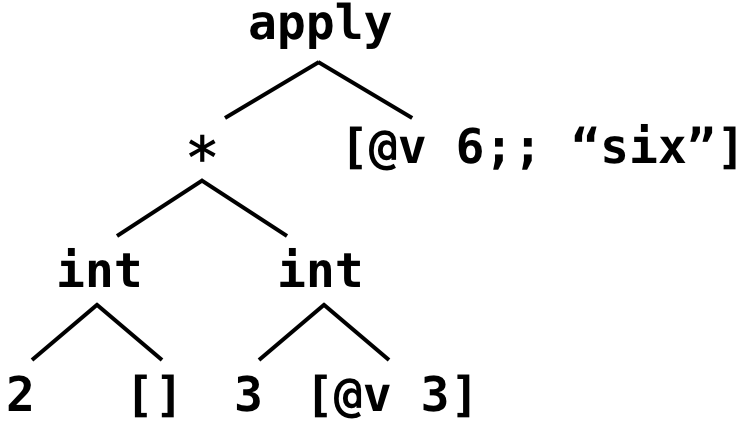
\includegraphics[width=5.2cm, height=3cm]{5/attribute.png}
  \end{center}
  \caption{attribute を含む構文木の例}
  \label{figure:attribute}
\end{figure}

OCaml のプログラムでは、任意の部分式に attribute をつけることができる。
式 \texttt{e} に OCaml プログラム \texttt{P} を引数に持つ
\texttt{name} という attribute を付けたものは \texttt{e[@name P ]} と書く。
例えば \texttt{(2 * 3[@v 3])[@v 6;; "six" ]} という式は大まかには図
\ref{figure:attribute} のように構文解析され、
ステッパプログラムのように構文木を扱うプログラムの中で
attribute の内容を利用することができる。
通常の OCaml コンパイラは attribute を無視するので、
シンタックスエラー等を起こしてしまう場合を除いて、
attribute が付いた式と付いていない式で意味は変わらない。

\begin{figure}
\begin{alltt}
  (* Step 0 *)                              (* Step 0 *)
  (2 * 3) + (5 * 7)[@stepper.redex ]        (2 * 3) + \colorbox{lightgreen}{(5 * 7)}
  (* Step 1 *)                              (* Step 1 *)
  (2 * 3) + 35[@stepper.reduct ]            (2 * 3) + \colorbox{purple}{35}
  (* Step 1 *)                              (* Step 1 *)
  (2 * 3)[@stepper.redex ] + 35             \colorbox{lightgreen}{(2 * 3)} + 35
  (* Step 2 *)                              (* Step 2 *)
  6[@stepper.reduct ] + 35                  \colorbox{purple}{6} + 35
  (* Step 2 *)                              (* Step 2 *)
  (6 + 35)[@stepper.redex ]                 \colorbox{lightgreen}{(6 + 35)}
  (* Step 3 *)                              (* Step 3 *)
  41[@stepper.reduct ]                      \colorbox{purple}{41}
\end{alltt}
\caption{ハイライトのための attribute の利用}
\label{figure:highlight}
\end{figure}

incremental でない OCaml ステッパでは、
各ステップで簡約が起こっている部分の式をハイライトして示すために
attribute を利用している。
例えば \texttt{(2 * 3) + (5 * 7)} というプログラムに対する
incremental でないステッパの出力は図 \ref{figure:highlight} の左の文字列である。
インタフェースを受け持つプログラムはこの文字列を受け取り、
図\ref{figure:highlight}の右側のように、
attribute が付いた式をハイライトし、
さらに attribute を表す文字列を削除した上で表示している。

本章の incremental なステッパでも、
同様の方法で簡約部分のハイライトを行う。
本論文では、ステッパの出力文字列中のハイライトのための attribute を省略したり、
緑色および紫色のハイライトで現すことがある。

\subsection{プログラムの attribute}
\label{OCamlのattribute-プログラムのattribute}
attribute はプログラム自体にも付けることができる。

OCaml のプログラムは structure item の列であり、
structure item には式、変数定義(\texttt{let 変数名 = 式})、
型定義、モジュール定義、attribute などの種類がある。
structure item の間には \texttt{;;} を書くことで明示的に structure item の境を示すことができる。

attribute の structure item はプログラム中に何度でも書くことができ、
名前の重複などに関する制約も無い。
また式に付ける attribute と同じく、
標準のコンパイラなどはこれを無視するのでプログラムの意味に影響を与えない。

\texttt{name} という名前で OCaml プログラム\texttt{P}
を含む attribute の structure item を \texttt{[@@@name P ]} と書く。
例えば \texttt{let a = 1 [@@@name1 1;; 2 + 3 ] let b = 2 [@@@name2 ]}
というプログラムは、
(1)\texttt{a} の定義、(2)\texttt{1} と \texttt{2 + 3}
を引数に持つ \texttt{name1} という attribute、(3)\texttt{b} の定義、
(4)引数なしの \texttt{name2} という attribute、
の4つの structure item のリストとして処理され、
それぞれの attribute の内容はステッパが参照することができる。

これを用いると、プログラムに自由に情報を付加することができる。
incremental なステッパの実装において、
副作用によって変化する「状態」や現在のステップ番号を記録するために使用している。


\section{生じる問題と解決方法}
\label{生じる問題と解決方法}

incremental でない OCaml ステッパと全く同じようにステップ出力を行うと、
incremental なステッパでは様々な問題が起きた。
本節ではその問題と、回避するために行った出力内容の変更について説明する。

\subsection{情報の消失}
\label{生じる問題と解決方法-情報の消失}

\subsubsection{問題点}
\label{生じる問題と解決方法-情報の消失-問題点}
\ref{ステッパの動作-DrRacketのステッパ} 節および \ref{ステッパの動作-incrementalでないOCamlステッパ} 節で紹介した既存のステッパは、ステップ実行をした結果を蓄えておき、ユーザが表示ステップを切り替える際にその中から表示するステップの情報を検索して表示するので、ステップ番号を指定すれば任意のステップをすぐに表示することができる。それに対して本研究で提案するステッパは、表示を切り替える命令が入力されるたびに1ステップ先や1ステップ前を計算することになる。その際のステッパの入力は前回出力したプログラムの一部である。すると、1ステップ前を計算する時に問題が起きる。

例えば、\texttt{2 * 3 + 5 * 7} というプログラムをステップ実行するとき、最初に表示される1ステップ目は\texttt{2 * 3 + 5 * 7 $\leadsto$ 2 * 3 + 35}であり、次ステップ表示命令が入力されると今度は \texttt{2 * 3 + 35} を入力として \texttt{2 * 3 + 35 $\leadsto$ 6 + 35} を出力する。ここで前ステップ表示命令が入力された時に、 \texttt{2 * 3 + 35} や \texttt{6 + 35} という情報から \texttt{2 * 3 + 5 * 7 $\leadsto$ 2 * 3 + 35} を導き出すことは不可能である。これは計算が不可逆的であるという性質によるものである。すなわち式 \texttt{5 * 7} と \texttt{35} のどちらからもその値が \texttt{35} だという情報は得られるが、式 \texttt{35} からそれがかつて \texttt{5 * 7} だったという情報は得られないのである。

\subsubsection{解決方法}
\label{生じる問題と解決方法-情報の消失-解決方法}

incremental なステッパでは、簡約後の式に簡約前の式の情報を、簡約された式を表す attribute \texttt{[@stepper.reduct ]} の引数として付加することで、簡約によって失われた情報を復元可能にする。「\texttt{式2} が簡約された結果の \texttt{式1}」を \texttt{式1[@stepper.reduct 式2]} と表して、\texttt{2 * 3 + 5 * 7 $\leadsto$ 2 * 3 + 35} の代わりに \texttt{2 * 3 + 5 * 7 $\leadsto$ 2 * 3 + 35[@stepper.reduct 5 * 7 ]}、また \texttt{2 * 3 + 35 $\leadsto$ 6 + 35} の代わりに \texttt{2 * 3 + 35[@stepper.reduct 5 * 7 ] $\leadsto$ 6[@stepper.reduct 2 * 3 ] + 35[@stepper.reduct 5 * 7 ]} を出力すると、どのステップの出力からでもオリジナルのプログラムまで情報を復元することができる。

さらに、直前のステップで簡約された式が明示的に分かるように、簡約された時のステップ番号も attribute に含める。例えば \texttt{6[@stepper.reduct 2 * 3 ] + 35[@stepper.reduct 5 * 7 ]} に \texttt{2 * 3} や \texttt{5 * 7} のそれぞれの簡約が行われた当時のステップ番号を追加して、\texttt{6[@stepper.reduct (2, 2 * 3) ] + 35[@stepper.reduct (1, 5 * 7) ]} と出力する。こうすると、ここから前のステップを求めるときに、最後に簡約されたのは \texttt{6} だとステップ番号から分かり、\texttt{6} をその attribute に記録された簡約前の式 \texttt{2 * 3} に置き換えることで前のステップ \texttt{2 * 3 + 35[@stepper.reduct (1, 5 * 7) ] $\leadsto$ 6[@stepper.reduct (2, 2 * 3) ] + 35[@stepper.reduct (1, 5 * 7) ]} が得られる。

\subsection{表示の崩れ}
\label{生じる問題と解決方法-表示の崩れ}
\subsubsection{問題点}
OCaml プログラムは、ライブラリで用意された関数を使うと文字列として出力することができ、本研究のステッパではその関数を利用する。その関数は、適当に改行やインデントを入れてプログラムを出力する。しかし、図\ref{figure:highlight} のように attribute が付いたプログラムを出力させて後から外部で attribute を消すと、プログラムの体裁が崩れてしまう可能性がある。

特に、\ref{生じる問題と解決方法-情報の消失-解決方法}節で示したように、簡約後の式に簡約前の式の情報を含む attribute を付けるようにしてステップ実行を進めると、attribute 付きの式の出力が複数行にわたってしまうことがある。すると、例えば
\begin{verbatim}
((2 * 3)
  [@reduct 長い式 ]) +
  (5 * 7)
\end{verbatim}
といった式の途中に改行が入った状態になり、外部のインタフェース用プログラムがこの文字列を受け取って
\begin{verbatim}
(2 * 3) + (5 * 7)
\end{verbatim}
と改行やスペースを調整して表示するのは難しい。

\subsubsection{解決方法}
\label{生じた問題と解決方法-表示の崩れ-解決方法}
我々は、実行に必要な情報がすべて含まれた式「処理用の式」と、表示するための整った式「表示用の式」をそれぞれ出力することでこれを解決した。

具体的には、\texttt{2 * 3 + 5 * 7} の最後のステップの出力が以下のようになるようにした。
\begin{verbatim}
  (* Step 2 *)
  [@@@stepper.process
    6[@stepper.reduct (2, 2 * 3) ] + 35[@stepper.reduct (1, 5 * 7) ] ]
  (6 + 35)[@x ]

  (* Step 3 *)
  [@@@stepper.process 41[@stepper.reduct (3,
    6[@stepper.reduct (2, 2 * 3) ] + 35[@stepper.reduct (1, 5 * 7) ] )] ]
  41[@t ]
\end{verbatim}
すなわち、
\begin{enumerate}
\item 処理用の簡約前の式(\texttt{[@stepper.reduct ]} を含む)を attribute に入れたもの
\item 表示用の簡約前の式(\texttt{[@x ]} を含む)
\item 処理用の簡約後の式(\texttt{[@stepper.reduct ]} を含む)を attribute に入れたもの
\item 表示用の簡約後の式(\texttt{[@t ]} を含む)
\end{enumerate}
の 4 つのプログラムを出力する。

「処理用の式」は前後のステップを計算するための情報を持つ式であり、そこまでの全ての簡約の情報を attribute に持つ。ユーザが見る画面には表示させないようにインタフェース側で処理をする。「表示用の式」はユーザに見せるための式であり、ハイライトをする式にのみ短い attribute が付いている。

余計な改行の原因である「簡約されている式をハイライトするための attribute」は、インタフェース側のプログラムが表示に利用するので完全に省略することはできない。そこで、上の例のように最も短い attribute \texttt{[@x ]}や \texttt{[@t ]} を簡約される式に付加することでハイライトする部分を示す。\texttt{x} と \texttt{t} はそれぞれ簡約基と簡約されたものを表す``redex''と``reduct''の略である。名前が 1 文字で他の情報を含まない attribute は文字数が少なくほとんどの場合改行を引き起こさないため、単純に attribute を文字列から削除してもユーザから見て不自然にプログラムの体裁が崩れることは少ないと考えられる。

次や前のステップを実行する際には、インタフェース側のプログラムが attribute である structure item \texttt{[@@@stepper.process ...]} の内容をステッパに渡すようにする。すると、ステッパには簡約の情報が全て含まれたプログラムが入力され、前のステップにも戻ることができる。前のステップの実行には処理用の簡約前の式、次のステップの実行には処理用の簡約後の式をステッパに渡す。


\section{$\lambda$計算に対する実装}

\begin{figure}
\begin{verbatim}
(* 式の種類の定義 *)
type expression_desc = Var of string                   (* x *)
                     | Fun of string * expression      (* λx. e *)
                     | App of expression * expression  (* e1 e2 *)
                              
and expression = {desc : expression_desc;  (* 式の内容 *)
                  attr : attribute list}   (* attribute [@name ... ] *)

and attribute = (string * payload)       (* 名前と内容のペア *)
and payload = (int * expression) option  (* ステップ番号と簡約前の式 *)
\end{verbatim}
\caption{対象言語の定義}
\label{figure:lambda}
\end{figure}

本節では、既存の OCaml ステッパ\cite{FSA18}の実装を紹介し、新しい OCaml ステッパの実装を示す。対象言語は型無しの$\lambda$式で、さらに実際の OCaml を模して任意の部分式に複数の attribute を付けられるものとするが、各 attribute の第一引数は attribute の名前とし、第二引数には\ref{生じる問題と解決方法-情報の消失-解決方法}節で定めた簡約の情報を簡単に表すために \texttt{Some (整数, 式)} または情報を持たないことを示す \texttt{None} のどちらか(\texttt{payload} 型)をとる\footnote{\texttt{[@x ]} は \texttt{("x", None)}、\texttt{[@stepper.reduct (1, 5 * 7)]} は \texttt{("stepper.reduct", Some (1, 5 * 7))} である。}。これらの型を図\ref{figure:lambda}のように定義する。式は \texttt{expression} 型であり、式本体の内容を表す \texttt{desc} と任意の個数の attribute を表す \texttt{attr} の2つの要素を持つ。

\subsection{incremental でないステッパ}

\begin{figure}[t]
\begin{spacing}{0.8}
  \begin{alltt}
\colorbox{lightgray}{(* コンテキストのフレームの定義 *)}
\colorbox{lightgray}{type frame = AppR of expr  (* e [.] *)}
\colorbox{lightgray}{           | AppL of expr  (* [.] v *)}

\colorbox{lightgray}{(* ステップ番号を格納する変数 *)}
\colorbox{lightgray}{let counter : int ref = ref 0}

(* 式\colorbox{lightgray}{とその周りのコンテキスト}を受け取って式を評価する *)
let rec eval (expr : expression) \colorbox{lightgray}{(context : frame list)} : expression =
  match expr.desc with
  | Var (x) -> failwith "error: Unbound variable"
  | Fun (x, f) -> expr
  | App (e1, e2) ->
    let arg\_value = eval e2 \colorbox{lightgray}{(AppR e1 :: context)} in         (* 引数部分を評価 *)
    let fun\_value = eval e1 \colorbox{lightgray}{(AppL arg\_value :: context)} in  (* 関数部分を評価 *)
    match fun\_value.desc with
    | Fun (x, f) ->
    let redex = \{desc = App (fun\_value, arg\_value);             (* 簡約前の式 *)
                 attr = expr.attr\} in
      let reduct = \{desc = (subst f x arg\_value).desc ;         (* 簡約後の式 *)
                    attr = expr.attr\} in
      \colorbox{lightgray}{memo redex reduct context;                              (* ステップ出力 *)}
      eval reduct \colorbox{lightgray}{context}                                 (* 簡約後の式を評価 *)
    | \_ -> failwith "error: not a function"

(* \colorbox{lightgray}{空のコンテキストで}式の評価を始める *)
let start (expr : expression) : expression = eval expr \colorbox{lightgray}{[]}
\end{alltt}
\end{spacing}
\caption{既存のステッパの実装}
\label{figure:old-stepper}
\end{figure}

incremental でないステッパは big-step インタプリタ関数に
ステップ出力のための作用を追加することで構築されている。
incremental でないステッパの実装は図\ref{figure:old-stepper}のようになる。
関数 \texttt{eval} は OCaml の call-by-value かつ right-to-left
の評価戦略に従った代入ベースの $\lambda$
計算のインタプリタにステップ実行のための作用を追加したステッパである。
背景に灰色が付いた部分がステップ実行のための作用であり、
白い部分のみを読むと単なるインタプリタとして見ることができる。
ただし関数 \texttt{subst} は代入の関数であり、
\texttt{subst f x arg\_value} は式 \texttt{f} の中の変数
\texttt{x} を式 \texttt{arg\_value} に置換した式を返す。
このステッパの出力は、
例えば入力プログラム \texttt{2 * 3 + 5 * 7} に対して、
図 \ref{figure:highlight} の左側の文字列(にステップ番号の表示を足したもの)である。

ステッパは実行可能なプログラムのみを受け付けるため、ステッパに渡される式の中に自由変数および型エラーは存在しない。さらにこのステッパの基となる代入ベースのインタプリタでは、関数の内部の式は必ず関数適用の簡約(すなわち実引数の代入)の後に実行するので、常に変数はその実行の前に束縛を解決されており、変数がインタプリタ関数の引数として実行されることはない。よって、関数 \texttt{eval} 中の \texttt{failwith} の呼び出しは起こり得ない。

\begin{figure}[t]
\begin{spacing}{0.8}
\begin{alltt}
(* 簡約前後の式とコンテキストを受け取って、そのステップを出力する *)
let memo (redex : expression) (reduct : expression) (context : frame list)
  : unit =
  let marked\_redex =                            (* 簡約前の式に attribute 追加 *)
    \{redex with attr = Some ("stepper.redex", None)\} in
  let marked\_reduct =                           (* 簡約後の式に attribute 追加 *)
    \{reduct with attr = Some ("stepper.reduct", None)\} in
  print\_counter ();                                 (* 簡約前ステップ番号を出力 *)
  print (plug redex current\_context);               (* 簡約前のプログラムを出力 *)
  counter := !counter + 1;                          (* ステップ番号を 1 増やす *)
  print\_counter ();                                 (* 簡約後ステップ番号を出力 *)
  print (plug reduct current\_context)               (* 簡約後のプログラムを出力 *)
\end{alltt}
\end{spacing}
\caption{ステップ出力関数}
\label{figure:memo}
\end{figure}

関数 \texttt{eval} の下から3行目の関数 \texttt{memo} は、簡約前のプログラムを出力し、 \texttt{counter} の値を1増やし、簡約後のプログラムを出力する関数である。その実装は図\ref{figure:memo}に示す。ただし、関数 \texttt{print\_counter : unit -> unit} はコメントとしてステップ番号 \texttt{(* Step n *)} を標準出力する関数、関数 \texttt{print : expr -> unit} は式を標準出力する関数、関数 \texttt{plug : expression -> frame list -> expression} は計算している途中の部分式とコンテキストを受け取って式を再構成する関数であり、実装は省略する。変数 \texttt{counter} には、現在のステップ番号が格納されている。式の評価中に関数適用の簡約を行うたびに1ずつ増加させることで、式全体の通しステップ番号を出力できる。


\subsection{incremental なステッパ関数}

\begin{figure}[t]
\begin{spacing}{0.8}
\begin{verbatim}
(* 実行の種類 *)
type mode = All | Next | Prev
let mode: mode =
  try (match Sys.getenv "STEPPER_MODE" with
    | "next" -> Next | "prev" -> Prev | _ -> All)
  with Not_found -> All

(* ステップ番号を格納する変数 *)
let counter: int ref =
  try int_of_string (Sys.getenv "STEPPER_COUNT")
  with Not_found -> match mode with All -> ref 0
                      | _ -> failwith "no step number"
\end{verbatim}
\end{spacing}
\caption{実行の種類とステップ番号の定義}
\label{figure:mode}
\end{figure}

incremental なステッパ関数では、たとえば入力 \texttt{2 * 3 + 35[@stepper.reduct (1, 5 * 7) ]} に対して、以下の3種類の処理を実装する。

\begin{itemize}
\item 全ステップ出力 \texttt{\colorbox{lightgreen}{2 * 3} + 35 $\leadsto$ \colorbox{purple}{6} + 35, \colorbox{lightgreen}{6 + 35} $\leadsto$ \colorbox{purple}{41}}
\item 次ステップ出力 \texttt{\colorbox{lightgreen}{2 * 3} + 35 $\leadsto$ \colorbox{purple}{6} + 35}
\item 前ステップ出力 \texttt{2 * 3 + \colorbox{lightgreen}{5 * 7} $\leadsto$ 2 * 3 + \colorbox{purple}{35}}
\end{itemize}

このうちどの処理を行うかは、図\ref{figure:mode}のように、
ステッパ関数のプログラムの実行ごとに環境変数で定めて、
\texttt{mode} というグローバル変数に格納する。

次ステップ出力の内容は全ステップ出力の冒頭の1ステップであるので、
もし前ステップ出力機能を実装しないならば、
例えば関数 \texttt{memo}(図\ref{figure:memo})の最後に
\begin{verbatim}
;if mode <> All then exit 0
\end{verbatim}
と書けばよい。すると mode が Next のときは最初のステップしか出力されず実行が終了し、
All のときは全ステップが出力される。

しかし、\ref{生じる問題と解決方法-情報の消失} 節で述べたように、
「前ステップ出力」処理のためには出力内容を増やしたり、
その新しい出力を処理できるようにしなければならない。
それぞれの処理において以下のような実装をする必要がある。
\begin{itemize}
\item 全ステップ出力:それを新しい入力として前ステップ出力は行わないので変更無し
\item 次ステップ出力:そのステップの簡約によって失われる情報を前ステップ出力で復元できるように attribute を付ける
\item 前ステップ出力:次ステップ出力時に attribute に書かれた情報から前ステップを導いて出力する
\end{itemize}

本研究では、incremental でないステッパにこれらの作用を更に付け足すことで、incremental なステッパを実装する。

\subsubsection{情報の付加}

\begin{figure}[t]
\begin{spacing}{0.8}
  \begin{alltt}
(* 簡約前後の式とコンテキストを受け取って、そのステップを出力する *)
let memo (redex : expression) (reduct : expression) (context : frame list)
  : unit =
  let marked_redex =                            (* 簡約前の式に attribute 付加 *)
    \{redex with attr = ("stepper.redex", None) :: redex.attr\} in
  let marked_reduct =
    \{reduct with
     attr = ("stepper.reduct",
             Some (!counter + 1,                 (* 簡約後の式にステップ番号と、 *)
                   redex))                           (* 簡約前の式の情報を追加 *)
            :: reduct.attr\} in
  if mode = Prev                                      (* 前ステップ出力のとき、 *)
  then counter := !counter - 1;                        (* ステップ番号を1戻す *)
  print_counter ();                                 (* 簡約前のステップ番号出力 *)
  print_as_attribute (plug redex context);        (* 処理用の簡約前のプログラム *)
  print (redex_mapper
           (plug marked_redex context));          (* 表示用の簡約前のプログラム *)
  counter := !counter + 1;                            (* ステップ番号を1進める *)
  print_counter ();                                 (* 簡約後のステップ番号出力 *)
  let latter_program = plug marked_reduct context in
  print_as_attribute (latter_program);            (* 処理用の簡約後のプログラム *)
  print (reduct_mapper latter_program);           (* 表示用の簡約後のプログラム *)
  if mode <> All then exit 0             (* 全ステップ実行でなければプロセス終了 *)
  \end{alltt}
  \end{spacing}
  \caption{incremental なステッパのための出力関数}
  \label{figure:new-memo}
\end{figure}

incremental でないステッパ関数では、例えば \texttt{(2 * 3) + (5 * 7)} に対して、2 ステップ目を
\begin{verbatim}
  (* Step 1 *)
  (2 * 3)[@stepper.redex ] + 35

  (* Step 2 *)
  6[@stepper.reduct ] + 35
\end{verbatim}
と出力するが、incremental なステッパでは \ref{生じる問題と解決方法}節で述べたように
\begin{verbatim}
  (* Step 1 *)
  [@@@stepper.process (2 * 3) + 35[@stepper.reduct (1, 5 * 7) ] ]
  (2 * 3)[@x ] + 35

  (* Step 2 *)
  [@@@stepper.process 6[@stepper.reduct (2, 2 * 3) ]
    + 35[@stepper.reduct (1, 5 * 7) ] ]
  6[@t ] + 35
\end{verbatim}
を出力したいので、出力をする関数 \texttt{memo} を書き換える必要がある。

図\ref{figure:memo} にある関数 \texttt{memo} の引数は簡約基、
それが簡約されたもの、その簡約時のコンテキストの 3 つであったが、
新しい出力の内容もこれらの情報から構成することができる。
その実装を図\ref{figure:new-memo}に示す。
関数 \texttt{print\_as\_attribute :\ expression -> unit} は、
\texttt{[@@@stepper.process ... ]} にプログラムを入れて出力する関数である。

ここで、\ref{生じる問題と解決方法-表示の崩れ}節で述べたように、表示用のプログラムではハイライトに最低限必要な attribute だけを出力したい。しかし、今簡約している式の外、すなわちコンテキストに含まれる式の中には attribute \texttt{[@stepper.reduct ]} が含まれうる。上の出力例で処理用
の \texttt{35} に付いている \texttt{[@stepper.reduct (1, 5 * 7) ]} がそれである。表示用のプログラムを出力するためには、今のステップで簡約される式以外の attribute を消したものを得る必要がある。

そのために、本研究では OCaml のモジュール Ast\_mapper を利用した。
Ast\_mapper は OCaml プログラムの構文木を簡単に部分的に変換するためのモジュールである。
ここでは詳しい紹介は省くが、
Ast\_mapper を利用して attribute のみを変換する関数
\texttt{redex\_mapper :\ expression -> expression} と関数
\texttt{reduct\_mapper :\ expression -> expression} を実装した。
\texttt{redex\_mapper} は \texttt{[@x ]} 以外の attribute を無くす変換をする関数であり、
\texttt{reduct\_mapper} は \texttt{[@stepper.reduct (今のステップ, 簡約前の式) ]} を
\texttt{[@t ]} にし、それ以外の attribute を無くす変換をする関数である。

以上によって、\ref{生じる問題と解決方法}節で定めたように、十分な情報を持つプログラムが出力できた。

\subsubsection{情報の利用}
簡約後の式に attribute が付加できたので、その情報を利用して「前ステップ出力」をする。前ステップ出力には、
\begin{enumerate}
\item 今のステップ番号を持つ attribute を探す
\item その attribute が付いた式を attribute 内の式に置換したプログラムを出力する
\end{enumerate}
という操作が必要となる。
「今のステップ番号を持つ \texttt{[@reduct ... ]}」は1つの式だけに付いており、
これを探すには式を全て探索する必要がある。
そのために、「前ステップ出力」時にだけ利用する新しいインタプリタ関数を作ってもよいが、
検索の順序はステッパ関数、すなわち図\ref{figure:old-stepper}の \texttt{eval} と同じなので、
本研究ではこの関数にさらに作用を足すことで前ステップ出力を行う。

\begin{figure}
\begin{spacing}{0.8}
\begin{alltt}
\colorbox{lightgray}{ (* 今のステップ番号の [@stepper.reduct] を探してその中の式を返す *)}
\colorbox{lightgray}{let rec find_last_reduct (attrs : attribute list) : expression =}
\colorbox{lightgray}{  match attrs with}
\colorbox{lightgray}{  | [] -> raise Not_found      (* リストの最後まで見つからなければ例外 Not_found *)}
\colorbox{lightgray}{  | ("stepper.reduct", Some (n, redex)) :: _        (* 簡約後のマークがあって、 *)}
\colorbox{lightgray}{    when n = !counter -> redex (* その番号が今のステップ番号だったらその式を返す *)}
\colorbox{lightgray}{  | _ :: rest -> find_last_reduct rest}

(* ステップ実行インタプリタ *)
let rec eval (expr : expression) (context : frame list) : expression =
\colorbox{lightgray}{  if mode = Prev}
\colorbox{lightgray}{  then begin try}
\colorbox{lightgray}{      let marked_redex = find_last_reduct expr.attr in}
\colorbox{lightgray}{      memo marked_redex expr                     (* 出力して最後に exit 0 する *)}
\colorbox{lightgray}{    with Not_found -> ()             (* expr が探している式でなければ何もせず、 *)}
\colorbox{lightgray}{  end;                                               (* 以下の match 文へ進む *)}
  match expr.desc with
    | Var (x) -> failwith "error: Unbound variable"
    | Fun (x, f) -> expr
    | App (e1, e2) ->
      let arg_value = eval e2 (AppR e1 :: context) in
      let fun_value = eval e1 (AppL arg_value :: context) in
      match fun_value.desc with                       (* 以下、次ステップの簡約 *)
        | Fun (x, f) ->
          let redex = \{expr with desc = App (fun_value, arg_value)\} in
          let reduct = \{(subst f x arg_value)
                        with attr = expr.attr\} in
          memo redex reduct context;
          eval reduct context
        | _ -> failwith "error: not a function"
\end{alltt}
\end{spacing}
\caption{incremental なステッパ関数}
\label{figure:new-stepper}
\end{figure}

前ステップ出力の処理は、関数 \texttt{memo} を図\ref{figure:new-memo}のように定義した上で図\ref{figure:new-stepper}のように実装することができる。灰色の部分が incremental になったことで加わった部分である。灰色の部分は、\texttt{if mode = Prev then begin ... end;} であることから分かるように、前ステップ出力モードの時にしか実行されない。

前ステップ出力モードの時の関数 \texttt{eval} の実行は、
まず今評価している式に
\texttt{[@stepper.reduct (今のステップ番号, 簡約前の式) ]}
が付いているかを調べることから始まる。
そこで見つかれば、その「 \texttt{簡約前の式} 」を利用して前ステップの出力をしてプロセスを終了する。
見つからなければ、\texttt{eval} の本体である \texttt{match} 文へ進む。
今評価している式をパターンマッチして、関数だったらそれ以上の簡約はできず、そのままその関数を返す。
関数適用だったら、引数部分の式の実行に移る。
するとまたその引数部分の式に
\texttt{[@stepper.reduct (今のステップ番号, 簡約前の式) ]}
が付いているかを調べる。あれば出力して終了、無ければ同様に式を普通に評価する。

このように実行を進めると、
1 以上の正しいステップ番号を変数 \texttt{counter} に持っている限り、
必ずどこかに \texttt{[@stepper.reduct (今のステップ番号, 簡約前の式) ]} が付いた式が見つかる。
そして、今のステップに至るまで行ってきた「次ステップの出力」と同じ順序で式を探索してきたため、
見つかるまでに評価した式は全て簡約済みであり、その式を見つけるまでに簡約処理、
すなわち \texttt{match fun\_value.desc with ...} を行うことは無い。
よって、灰色の部分を書き足すことで前ステップ出力が可能になる。

以上のように、incremental でないステッパ関数
(図\ref{figure:old-stepper}, \ref{figure:memo})
を図\ref{figure:mode}, \ref{figure:new-memo}, \ref{figure:new-stepper}のように書き換えることで、
incremental なステッパ関数を実装できる。


\subsection{実際のステッパ}
\label{実装-実際のステッパ}

実際に著者らが実装するステッパは、対象を OCaml の一部としており、以下の構文に対応している(一部は開発中である)。
\begin{itemize}
\item 整数、実数、真偽値、文字、文字列、リスト、組、レコード、ユーザ定義型
\item 条件分岐、変数定義、再帰関数定義、パターンマッチ、例外処理
\item List モジュール、ユーザ定義モジュール
\item 配列、逐次実行、標準出力関数(開発中)
\end{itemize}

副作用に関わる構文について、incremental でないステッパ\cite{FSA18}ではステッパプロセスが書き換え可能な変数の値や標準出力された文字列を保持することができたが、incremental にすることでそれが不可能になるので、プログラムの attribute を用いてそのような情報もステップ出力に含めるようにすることで実装することを目指している。

\begin{figure}
  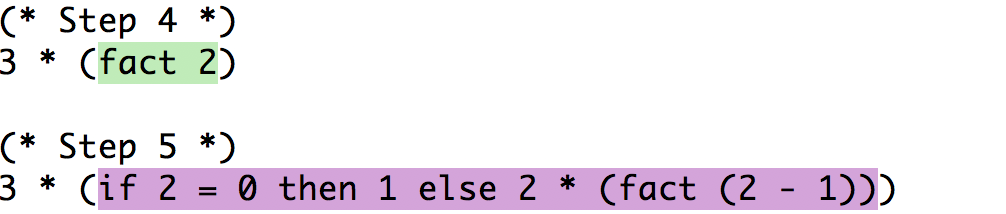
\includegraphics[height=2cm]{5/skip1.png}
  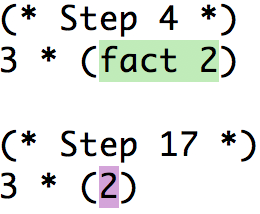
\includegraphics[height=2cm]{5/skip2.png}
  \caption{ステッパのスキップ機能}
  \label{figure:skip}
\end{figure}

また、著者らの incremental でないステッパ\cite{FSA18}は、プログラムの流れを理解する助けやステッパの利便性の向上のため、関数適用式が値に計算されるまでが1ステップであるかのように進める機能を有していた。図\ref{figure:skip} の左のように関数適用が簡約されるステップで Skip ボタンを押すと、図\ref{figure:skip} 右のように、下のプログラムが「関数適用式が値に簡約されたステップ」のプログラムに変わる。この状態で Next ボタンを押すとその続き、図\ref{figure:skip} の場合には \texttt{3 * 2 $\leadsto$ 6} のステップが表示される。これを本研究の incremental なステッパでも1ステップとして扱い、1度の実行で関数適用が値になるステップまでを計算し、その最後のステップを出力するように実装を進めている。そのためには、図\ref{figure:mode} の \texttt{mode} 型にスキップのためのコンストラクタを追加し、そのモードの場合には「実行している関数適用式が値になるステップまでは出力・終了を行わない」ようにするだけで良い。


\subsection{ツールの実装}

ここまで、ステッパ関数としてのステッパプログラムの実装を紹介した。
ユーザが incremental なステッパツールを使用するには、
ユーザの入力を受けてステッパプログラムを呼び出しステップを表示する外部のプログラムが必要になる。

DrRacket のステッパ\cite{clements01}や incremental でない OCaml ステッパでは、
外部のプログラムは「ステッパを起動して、出力を蓄えて、ユーザの操作に従って表示」をしていたが、
本研究のステッパでは、
「ユーザの操作に従ってステッパを呼び出して、出力されたものを装飾して表示」をする。
すると、外部のプログラムではステップ番号と前回の出力のみを保持することで実装が可能になる。


\section{予想される問題点とその経過}
本節では、incremental な OCaml ステッパを実際に利用するときに発生しうる問題点とその解決方法を挙げ、
大学の授業 ( \ref{section:experiment__course} 節で触れる) で利用してそれらが実際に問題になったかどうかを述べる。

\subsection{文字数の爆発}
\label{予想される問題点-文字数の爆発}

\subsubsection{問題点}

本章のステッパでは、
任意のステップの「処理用の出力」に入力プログラムからそこまでの簡約の過程が記されているため、
1ステップ進むごとに文字数が増加する。
具体的には、簡約基 \texttt{e1} が式 \texttt{e2} に簡約されるステップでは、
その時点のコンテキストを \texttt{E}、ステップ番号を \texttt{n} とすると、
簡約前のプログラムが \texttt{E[e1]}、
簡約後のプログラムが \texttt{E[e2[@stepper.reduct n;; e1]]} となる。
\texttt{E} の文字数は変わらないので、\texttt{e2[@stepper.reduct n;;}
と \texttt{]}の分の文字数が増加することになる。
これを続けていくと、1ステップあたり少なくとも22文字は増加することになり、
仮に百万ステップの簡約をするとプログラムは数千万文字になる。
すると、毎ステップの入出力や通信に時間がかかる可能性がある。

\subsubsection{解決方法}

解決策としては、古いステップの attribute は削除してしまうという方法が考えられる。
たくさんのステップを見てから最初の方のステップまで戻るユーザは少ないと仮定すれば、
ある程度前のステップについての attribute があったら、
関数 \texttt{memo} で出力するプログラムを再構成する際に消去すれば、
さほど実際の使用に影響なく出力する文字数を減らすことができる。

\subsubsection{使用した結果}

実際の incremental な OCaml ステッパ (\ref{実装-実際のステッパ} 節) では、
Emacs Lisp プログラムによってステッパ関数の実行や表示を制御する。
これを用いた授業では、文字数の多さが原因の不具合は報告されず、
1 ステップの入出力にかかる時間も利用に支障が出ない程度だった。

\subsection{実行時間}
\label{予想される問題点-実行時間}

\subsubsection{問題点}

ステップ数が膨大になると、後ろの方までステップ実行をするのは困難である。
incremental なステッパ関数での実行速度は通常の OCaml 処理系に決して及ばないので、
1ステップずつ進める場合でも、スキップ機能(\ref{実装-実際のステッパ}節)を使う場合でも、
実行を多く進めるには長い時間が掛かってしまう。

\subsubsection{解決方法}
少しでも急ぐ為には、一般的なデバッガのように、
ステップ実行したい式の付近にユーザがブレークポイントを設定して、
そこからステップ実行を始めるという方法が考えられる。
そのためには、ブレークポイントまでを部分的に native code にコンパイルして実行するなどの方法を取らざるを得ない。
しかしいずれにしても、
通常の OCaml コンパイラを用いても長時間かかるプログラムの実行を早く終わらせることは不可能である。

\subsubsection{使用した結果}

1 ステップずつ進める場合は、プログラムの実行を後ろの方まで進めることは困難であるが、
ステップごとの実行時間が問題になることはなかった。
スキップ機能を使用する場合は、やはり通常の OCaml で実行するよりも長い時間を要した。
具体的には、東京メトロ全線の駅についてダイクストラ法で最短路問題を解くプログラムの実行に、
通常の OCaml では 0.327 秒、incremental な OCaml ステッパではスキップ機能を使用して約 54 秒かかった。

\subsection{関数適用評価スキップ後の前ステップ出力}

\subsubsection{問題点}

関数適用をスキップ(\ref{実装-実際のステッパ}節)した後に前のステップに戻ろうとすると、
スキップで飛ばされたステップには戻ることができない。
たとえば図\ref{figure:skip}のように2の階乗の計算をスキップしたとすると、
図\ref{figure:skip}の右の状態から、incremental でないステッパでは
\begin{itemize}
\item スキップをする前の関数適用式が簡約されるステップ5(図\ref{figure:skip}左)
\item 関数適用式が最終的な値になるステップ17(
\texttt{3 * \colorbox{lightgreen}{(2 * 1)} $\leadsto$ 3 * \colorbox{purple}{2}})
\end{itemize}
のどちらにも戻ることができたが、incremental なステッパでは前者にしか戻ることができない。

その原因は、incremental でないステッパでは \ref{予想される問題点-実行時間}
節で述べたように文字列検索によってステップ表示を切り替えていたので任意のステップに移ることができたのに対して、
incremental なステッパではステッパ関数が関数適用式が値になるまでを1ステップとして出力し、
その間の簡約についての情報は出力しないからである。

\subsubsection{解決方法}

これを解決するには、
スキップする部分の計算をしている間の簡約についても attribute に情報を蓄え、
スキップ後のステップで全ての簡約の情報が入った長いプログラムを出力する必要がある。
しかしそのようにすると
\ref{予想される問題点-文字数の爆発} 節と
\ref{予想される問題点-実行時間} 節の問題がより深刻になる可能性がある。

\subsubsection{使用した結果}

ステッパを利用した学生に答えてもらったアンケートに
「ステッパの不便なところ、欲しい機能などがあれば教えてください。」
という質問を含めたが、この点に関する要望は出なかった。


\section{この章のまとめ}

本研究では、
OCaml の一部の構文に対するステッパを、
1度の実行で1つの簡約のみを行うように変更し、
ステッパの起動時間を短縮した。
そのためには任意のステップのプログラムから
それ以前のステップのプログラムを計算できるようにする必要が生まれたので、
それまでの簡約の内容を全て記録したプログラムを出力することで
入力プログラムの情報が失われないようにした。


\chapter{評価}
\label{chapter:experiment}

% \section{はじめに}
% \label{section:experiment__intro}
% セクションにする意味なかったか

2016 年度から 2018 年度の間、
我々は \ref{section:ocaml stepper} で述べた OCaml ステッパを
% Since 2016, we have been using (earlier versions of) our stepper in an
% introductory OCaml course called ``Functional Programming'',
% taught by the third author at Ochanomizu University.
お茶の水女子大学で毎年前期に開講されている授業「関数型言語」において利用してきた。
この章では、授業で実際に学生に OCaml ステッパを使ってもらったことで
得られた実行ログやアンケート結果からステッパの教育的効果について考察する。

まず \ref{section:experiment__course} 節で
ステッパを使用した授業の内容や進め方について説明する。
そして \ref{section:experiment__result} 節でステッパの効果について考察する。


\section{実際に使用したステッパ}
\label{section:experiment__stepper}

我々が実装した OCaml ステッパは、
\ref{section:try-with__stepper} 節で示した try-with と比べて
以下のような特徴がある。

\begin{itemize}
\item 型エラー等を想定しない。
\item 授業「関数型言語」で使用する構文のほぼ全てに対応している。
\item 関数適用が $\beta$ 簡約されるステップからその式が値になるステップまで飛ばす機能がある。
\end{itemize}

この節ではそれぞれについて述べる。

\subsection{型エラーについて}
\label{subsection:stepper__type}

OCaml ステッパでは、
まず入力プログラムを OCaml のパーザを利用して構文木にし、型チェックをする。
未定義変数エラーを含むシンタックスエラーや型エラーになった場合は
ステッパ本体のプログラムを起動せず、OCaml が示すエラーメッセージを表示する。
よって、コンパイルエラーがあるプログラムの構文木がステッパ関数に渡されることは無いという
仮定の上で実装されている。
ゼロ除算等の実行時エラーに関しては OCaml では例外の発生として処理されるので、
そのようにステップ実行処理を続行する。
ただし、例外が捕捉されないままその文の実行が終わってしまった場合はそこでステップ実行を終了する。

\subsection{対象構文}
\label{subsection:stepper__syntax}
% In Figure \ref{figure:ocamlstep},
% we show a reduction sequence produced by the actual stepping evaluator.
% 我々が実装した OCaml ステッパが出力するステップ列の例を図 \ref{figure:ocamlstep} に示す。
% The evaluator supports the following syntactic constructs:
このステッパは以下の構文に対応している。

\begin{itemize}
% \item integers, floating point numbers, booleans, characters, strings
% \item lists, tuples, records
% \item user-defined datatypes
% \item conditionals, let-expressions, recursive functions, pattern-matching
% \item exception handling operators
% \item printing functions and sequential execution
% \item the List module, user-defined modules
% \item references, arrays
\item 整数、実数、真偽値、文字、文字列型
\item リスト、組、レコード
\item ユーザ定義型
\item 条件分岐、変数定義、再帰関数定義、パターンマッチ
\item List モジュール、ユーザ定義モジュール
\item 例外処理
\item 標準出力関数、逐次実行
\item 書き換え可能な変数、配列
\end{itemize}

標準出力や書き換え可能な変数を含むプログラムでは、
標準出力された文字列や変数に格納された値などの「状態」をインタプリタが保持する必要がある。
状態の情報はステッパプログラム内の書き換え可能なグローバル変数の中に格納することで実装した。

\begin{figure}
  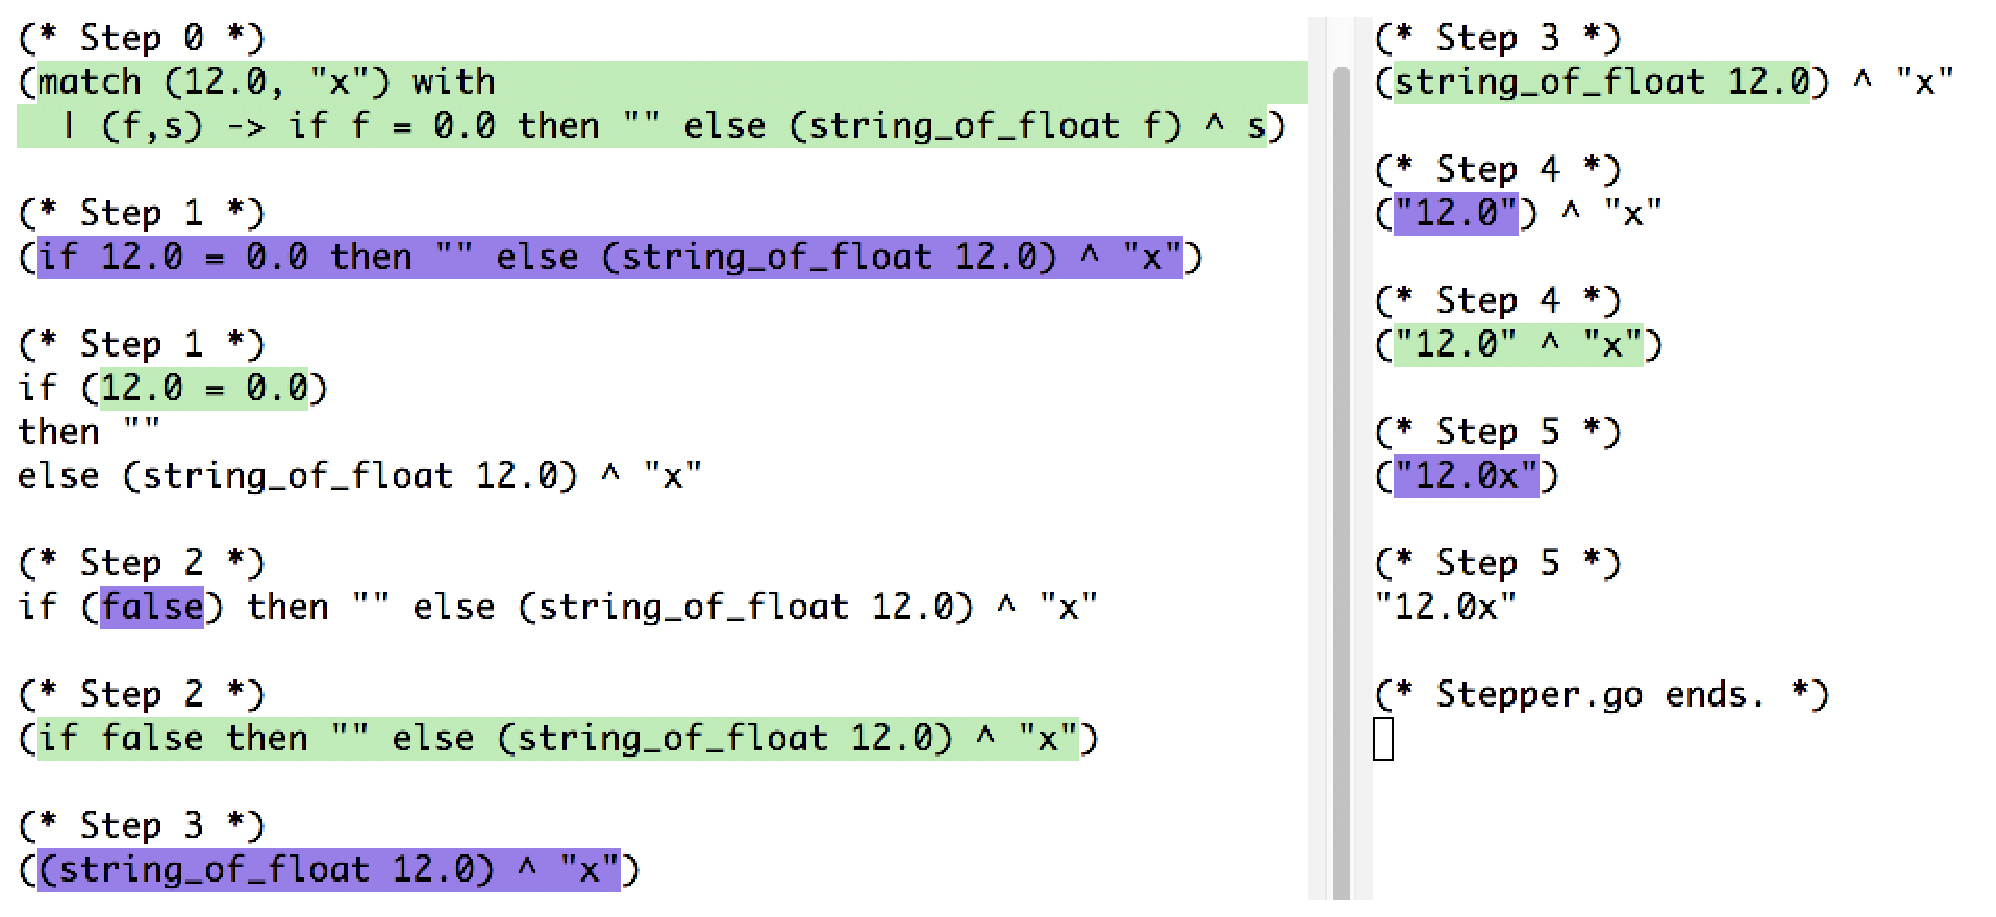
\includegraphics[width=14cm]{6/longexample.eps}
%   \caption{Evaluating programs using the actual stepper}
  \caption{実際のステッパでプログラムを実行する様子}
  \label{figure:ocamlstep}
\end{figure}

OCaml ステッパは他に授業で利用する一部の演算子などに対応している。
図 \ref{figure:ocamlstep} に実際のステップ列の例を示す。

% ref、配列を使うやつにする?

\subsection{関数適用のスキップ}
\label{subsection:skip}

\begin{figure}
  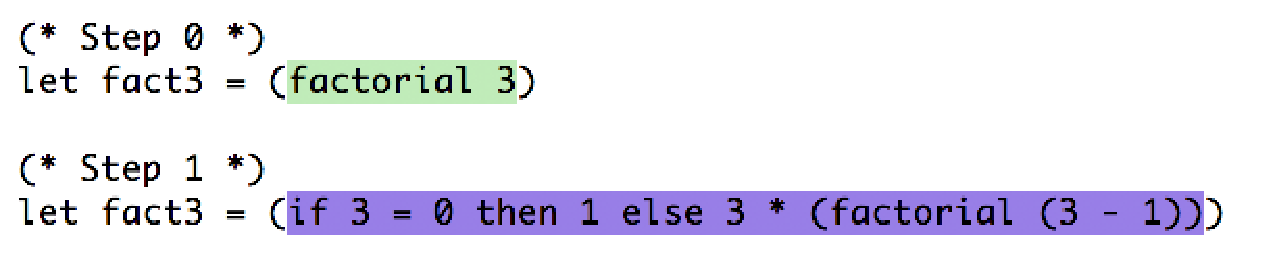
\includegraphics[width=10cm]{6/beforeskip.eps}
  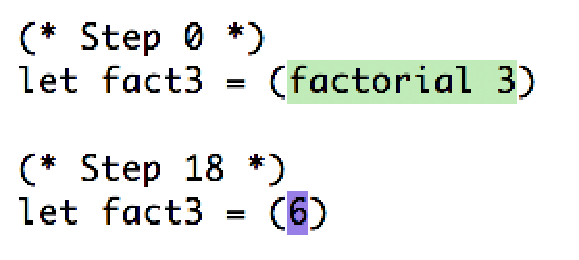
\includegraphics[width=4.3cm]{6/afterskip.eps}
%   \caption{Skipping evaluation of the factorial function}
  \caption{階乗関数をスキップする様子}
  \label{figure:factskip}
\end{figure}

% To allow the user to adjust granularity of steps,
% we provide an option for skipping
% the evaluation of the current function application.
プログラムのステップ数が多くなると、デバッグの目的でステップ実行をするときに
膨大な計算ステップを1つ1つ追って見るのは効率が悪く、
次第に実用に耐えるものではなくなってしまう。
そこで本研究では、「関数適用」を基準としてステップを飛ばす機能を追加した。

% Let us look at Figure \ref{figure:factskip},
% which shows skipping of the factorial function.
図 \ref{figure:factskip} に、階乗関数のスキップの様子を示す。
% By pressing the ``skip'' button,
% we can directly go from the program on the left to the one on the right,
% without seeing the intermediate steps that appear
% during the evaluation of the function's body.
左の状態で「skip」ボタンを押すと、関数の中身
\texttt{if 3 = 0 then 1 else 3 * (factorial (3 - 1))} が
\texttt{6} になるまでの実行ステップを見ることなく右の画面に移ることができる。
% This feature helps us focus on the steps we are interested in,
% allowing us to grasp the overall flow of the execution.
これによって見たいステップだけに注目することができ、実行の全体の流れを把握しやすくなる。

% The skipping feature requires some modifications to
% the \texttt{eval} function (Figure \ref{figure:skipapp}).
このスキップ機能は、
\ref{chapter:try-with} 章で try-with に対応したステッパ
(図 \ref{figure:stepper}) の eval 関数を
図 \ref{figure:skipapp} のように変更することで実装できる。
% The idea is to sandwich the steps within an application between two strings:
本研究では、飛ばすステップ列を
% \texttt{(* Application n start *)} and \texttt{(* Application n end *)}.
\texttt{(* Application n start *)} と \texttt{(* Application n end *)}
という 2 つの文字列で挟む方法をとった。
% Here, \texttt{n} tells us at which step we have entered the application.
\texttt{n} は関数適用の実行が始まるステップの番号である。
あるステップで実行が始まる関数適用は必ず 1 つ以下なので、
このステップ番号によって関数適用を一意に特定することができる。
% These strings are printed using the \texttt{apply\_start} and
% \texttt{apply\_end} functions,
% and help the Emacs Lisp program to hide unnecessary steps.
関数 \texttt{apply\_start :\ unit -> int} が前者を出力する関数、
関数 \texttt{apply\_end : int -> unit} が後者を出力する関数である。
表示処理をする Emacs Lisp プログラムがこれらの文字列を検索し、
間のステップを隠す処理をする。
% We show an example output sequence in Figure \ref{figure:skipping}.
スキップ機能を追加したステッパ関数の出力は例えば図 \ref{figure:skipping} のようになる。

\begin{figure}
\begin{alltt}
let rec eval expr ctxt = match expr with
    ...
  | App (e1, e2) ->
    begin
      let v2 = eval e2 (add ctxt (CAppR e1)) in
      let v1 = eval e1 (add ctxt (CAppL v2)) in
      match v1 with
      | Lam (x, e) ->
        let e' = subst e x v2 in
        \colorbox{lightgray}{let apply_num = apply_start () in}                (* output start mark *)
        memo (App (v1, v2)) e' ctxt;
        let v = eval e' ctxt in
        \colorbox{lightgray}{apply_end apply_num;}                               (* output end mark *)
        v
      | _ -> failwith "not a function"
    end
  | ...
\end{alltt}
\caption{関数適用をスキップするためのステッパ関数}
\label{figure:skipapp}
\end{figure}

\begin{figure}
\texttt{(* Step 0 *) (f 4) + \colorbox{lightgreen}{10 * 100}\\
(* Step 1 *) (f 4) + \colorbox{purple}{1000}\\
(* Application 1 start *)\\
(* Step 1 *) \colorbox{lightgreen}{f 4} + 1000\\
(* Step 2 *) \colorbox{purple}{(4 * 2) - 1} + 1000\\
(* Step 2 *) \colorbox{lightgreen}{(4 * 2} - 1) + 1000\\
(* Step 3 *) \colorbox{purple}{(8} - 1) + 1000\\
(* Step 3 *) \colorbox{lightgreen}{8 - 1} + 1000\\
(* Step 4 *) \colorbox{purple}{7} + 1000\\
(* Application 1 end *)\\
(* Step 4 *) \colorbox{lightgreen}{7 + 1000}\\
(* Step 5 *) \colorbox{purple}{1007}}
\caption{関数適用をスキップするためのステッパの出力}
\label{figure:skipping}
\end{figure}


\section{授業の内容}
\label{section:experiment__course}
% The ``Functional Programming'' course teaches
% how to program with functions and types, covering
% basic topics such as recursion, datatypes, effects, and modules.
「関数型言語」は OCaml を用いて関数型プログラミングを学ぶ授業であり、
再帰、データ型、副作用、モジュールなどの基本的な言語機能を扱う。
% The course consists of 15, weekly lab sessions, and each session
%  consists of 90 minutes lab-style class per week.
学期全体を通して、学生はダイクストラ法に基づいて最短路問題を解くプログラムを作成する。
授業は週に1回、90分間で、全15回で構成されている。
% (Many students remain in the lab after 90 minutes up until around 150
% minutes.)
(授業終了後も教室に残って作業を続ける学生も多い。)
% Throughout the course, students build a program that searches for
% the shortest path based on Dijkstra's algorithm.
% The participants of the course are second-year undergraduate students
% majoring in computer science (around 40 students each year).
% All students enter this course after a CS 1 course in the C
% programming language.
受講者は情報科学を専攻する学部2年生で、毎年40人程度である。
全ての学生がこの授業より前にC言語によるプログラミングを経験している。

% The course is taught in a ``flipped classroom'' style.
この授業では「反転授業」を行なっている。
反転授業とは、学生が各自内容を予習し、授業時間は講義を行わず演習などに活用する授業形態である。
% Before every meeting, students are asked to study assigned readings
% and videos prepared by the instructor and answer simple quizzes.
この授業では、学生は毎週の授業の前に、この授業に向けた教科書 \ref{Asai07} と教員が作成した動画による予習をし、
インターネット上で数問の簡単な問題に解答する。
% In the classroom, they practice the newly covered topics
% through exercises, with assistance of the instructor as well as five
% to six teaching assistants (including the first and second authors).  
授業時間内には、学生はその回に新しく取り上げた内容に関する演習問題に取り組み、
教員および5〜8人のティーチングアシスタントに質問することができる。

% The exercises include simple practice problems and report problems.
演習問題はほとんどが要求を満たす関数を実装するというものであり、
「練習問題」と「レポート課題」に分かれている。
% The former are for confirming students' understanding of the
% topics and are expected to be completed within a class.
練習問題は学生がどの程度その回の内容を理解しているか確認するための簡単な問題で、
授業時間内に解くことを期待している。
% The latter problems (for credit) are due in one week.
レポート課題は評定に利用する問題■■で、締め切りが1週間後に設定されている。

授業をする演習室では常に OCaml プログラム実行のログをとっている。
% Whenever a student executes a program, by either step execution or
% standard execution, the program as well as its execution log (syntax
% errors, type errors, or the result of execution) are recorded.
学生がプログラムを実行する時には必ず、ステッパによる実行と通常の実行のどちらも、
プログラム全文と実行ログが記録される。

% For most of the problems (up to the 12th week), we provide a check system
% where students can submit their solutions to see whether they pass the
% given tests.
解答プログラムが合っているかどうかを確認する方法の 1 つとして、
「チェックシステム」を用意してある。
チェックシステムは教員が用意した単体テストに通るかどうかを確認できるプログラムで、
問題ごとに用意されており、12 週目までのほとんどの問題を対象にしている。
各学生が各問題のチェックシステムに初めて通った時には学生の ID が記録されるようになっており、
% To earn points for report problems, students are required to have their
% programs pass the check system.
締め切りまでに 1 度以上チェックシステムに通ることが、レポート課題の各問で点を得る条件に含まれている。


\section{結果}
\label{section:experiment__result}

ステッパの学習的効果を評価するため、我々は以下の項目について調査した。

\begin{itemize}
\item ステッパがどれほど使われていたか
\item ステッパをよく使った年と使わなかった年で学生の解答の速さに違いがあったか
\item 学生がステッパについてどう感じたか
\end{itemize}

ステッパがどれほど使われたかについては、 OCaml 実行ログからステッパによる実行とそうでない実行の数を数えた。
解答の速さの差は、チェックシステムに記録されている時刻、
すなわち学生が初めて正解のプログラムをチェックシステムに通した時刻から統計的に分析した。
最後の項目については、学生にアンケートを取った。

% \subsection{The Uses of the Stepper}
\subsection{ステッパの使用状況}
\label{subsection:result__uses}

% We introduced the stepper into Functional Programming in 2016.
我々が授業「関数型言語」にステッパを導入したのは 2016 年度である。
% Although the steppers used in the past had
% almost the same user-interface as the one shown
% in Figure \ref{figure:ocamlfac}, they differ in the following ways:
ステッパのインタフェースは2016年度から2018年度まで概ね変わらない (図 \ref{figure:ocamlfac}) が、
以下の点で各年度のステッパの機能は異なる。
\begin{description}
% \item[2016] This first version supported function definitions,
% conditionals, records, lists, and recursion.  However, there were
% various operations that were not supported.
% As such, the usability of the stepper was low.
\item[2016年度] 関数定義、条件分岐、レコード、リスト、再帰のような
非常に基本的な式と一部の演算子のみが実行できるステッパを利用した。
% Moreover, when the instructor introduced the stepper to students, he
% only mildly encouraged to use it.
また、教員がステッパを学生に紹介する際に、ステッパの使用を強くは奨励しなかった。
% Although we do not know how much the stepper was used in 2016 since we
% did not log the execution of stepper, we expect it was used
% only rarely in the first few weeks of the course.
2016 年度はステッパによるプログラム実行のログを採取していなかったため
ステッパがどれくらい利用されていたのかは不明であるが、
最初の数週にわずかに利用されたのみだと我々は考えている。
% \item[2017] Based on the lessons from the previous year, the second
% version supported most operations used in the first six weeks.
\item[2017年度] 6 週目までに学習する構文要素のほとんどに対応したステッパを利用した。
% The instructor introduced the stepper up front at the first class and
% showed how to use the stepper with various examples in the subsequent
% classes.
教員は最初の授業で事前にステッパを紹介し、
その後の授業でも様々な例でステッパを利用して見せた。
% \item[2018] The third version supported almost all the constructs
% needed for the course, including modules, exception handling,
% sequential execution, printing, references, and arrays.
\item[2018年度] \ref{figure:ocamlfac} 節で紹介した、
モジュール、例外処理、逐次実行、配列などを実行できるステッパを利用した。
これは授業範囲のほとんどの構文要素を含んでいる。
% It also supported skipping of function application.
また関数適用のスキップ機能も追加した。
% The instructor introduced the stepper as though the stepper was the
% only way to execute OCaml programs, encouraging the uses of the
% stepper.
教員は、まるでステッパでしかプログラムが実行できないかのように学生に紹介することで、
学生にステッパの利用を促した。
% (Students gradually realized that they could execute a program in the
% interpreter in a few weeks.)
(数週の間に学生は普通のインタプリタで実行ができることにだんだん気付いていった。)
\end{description}

\begin{figure}
  \begin{center}
    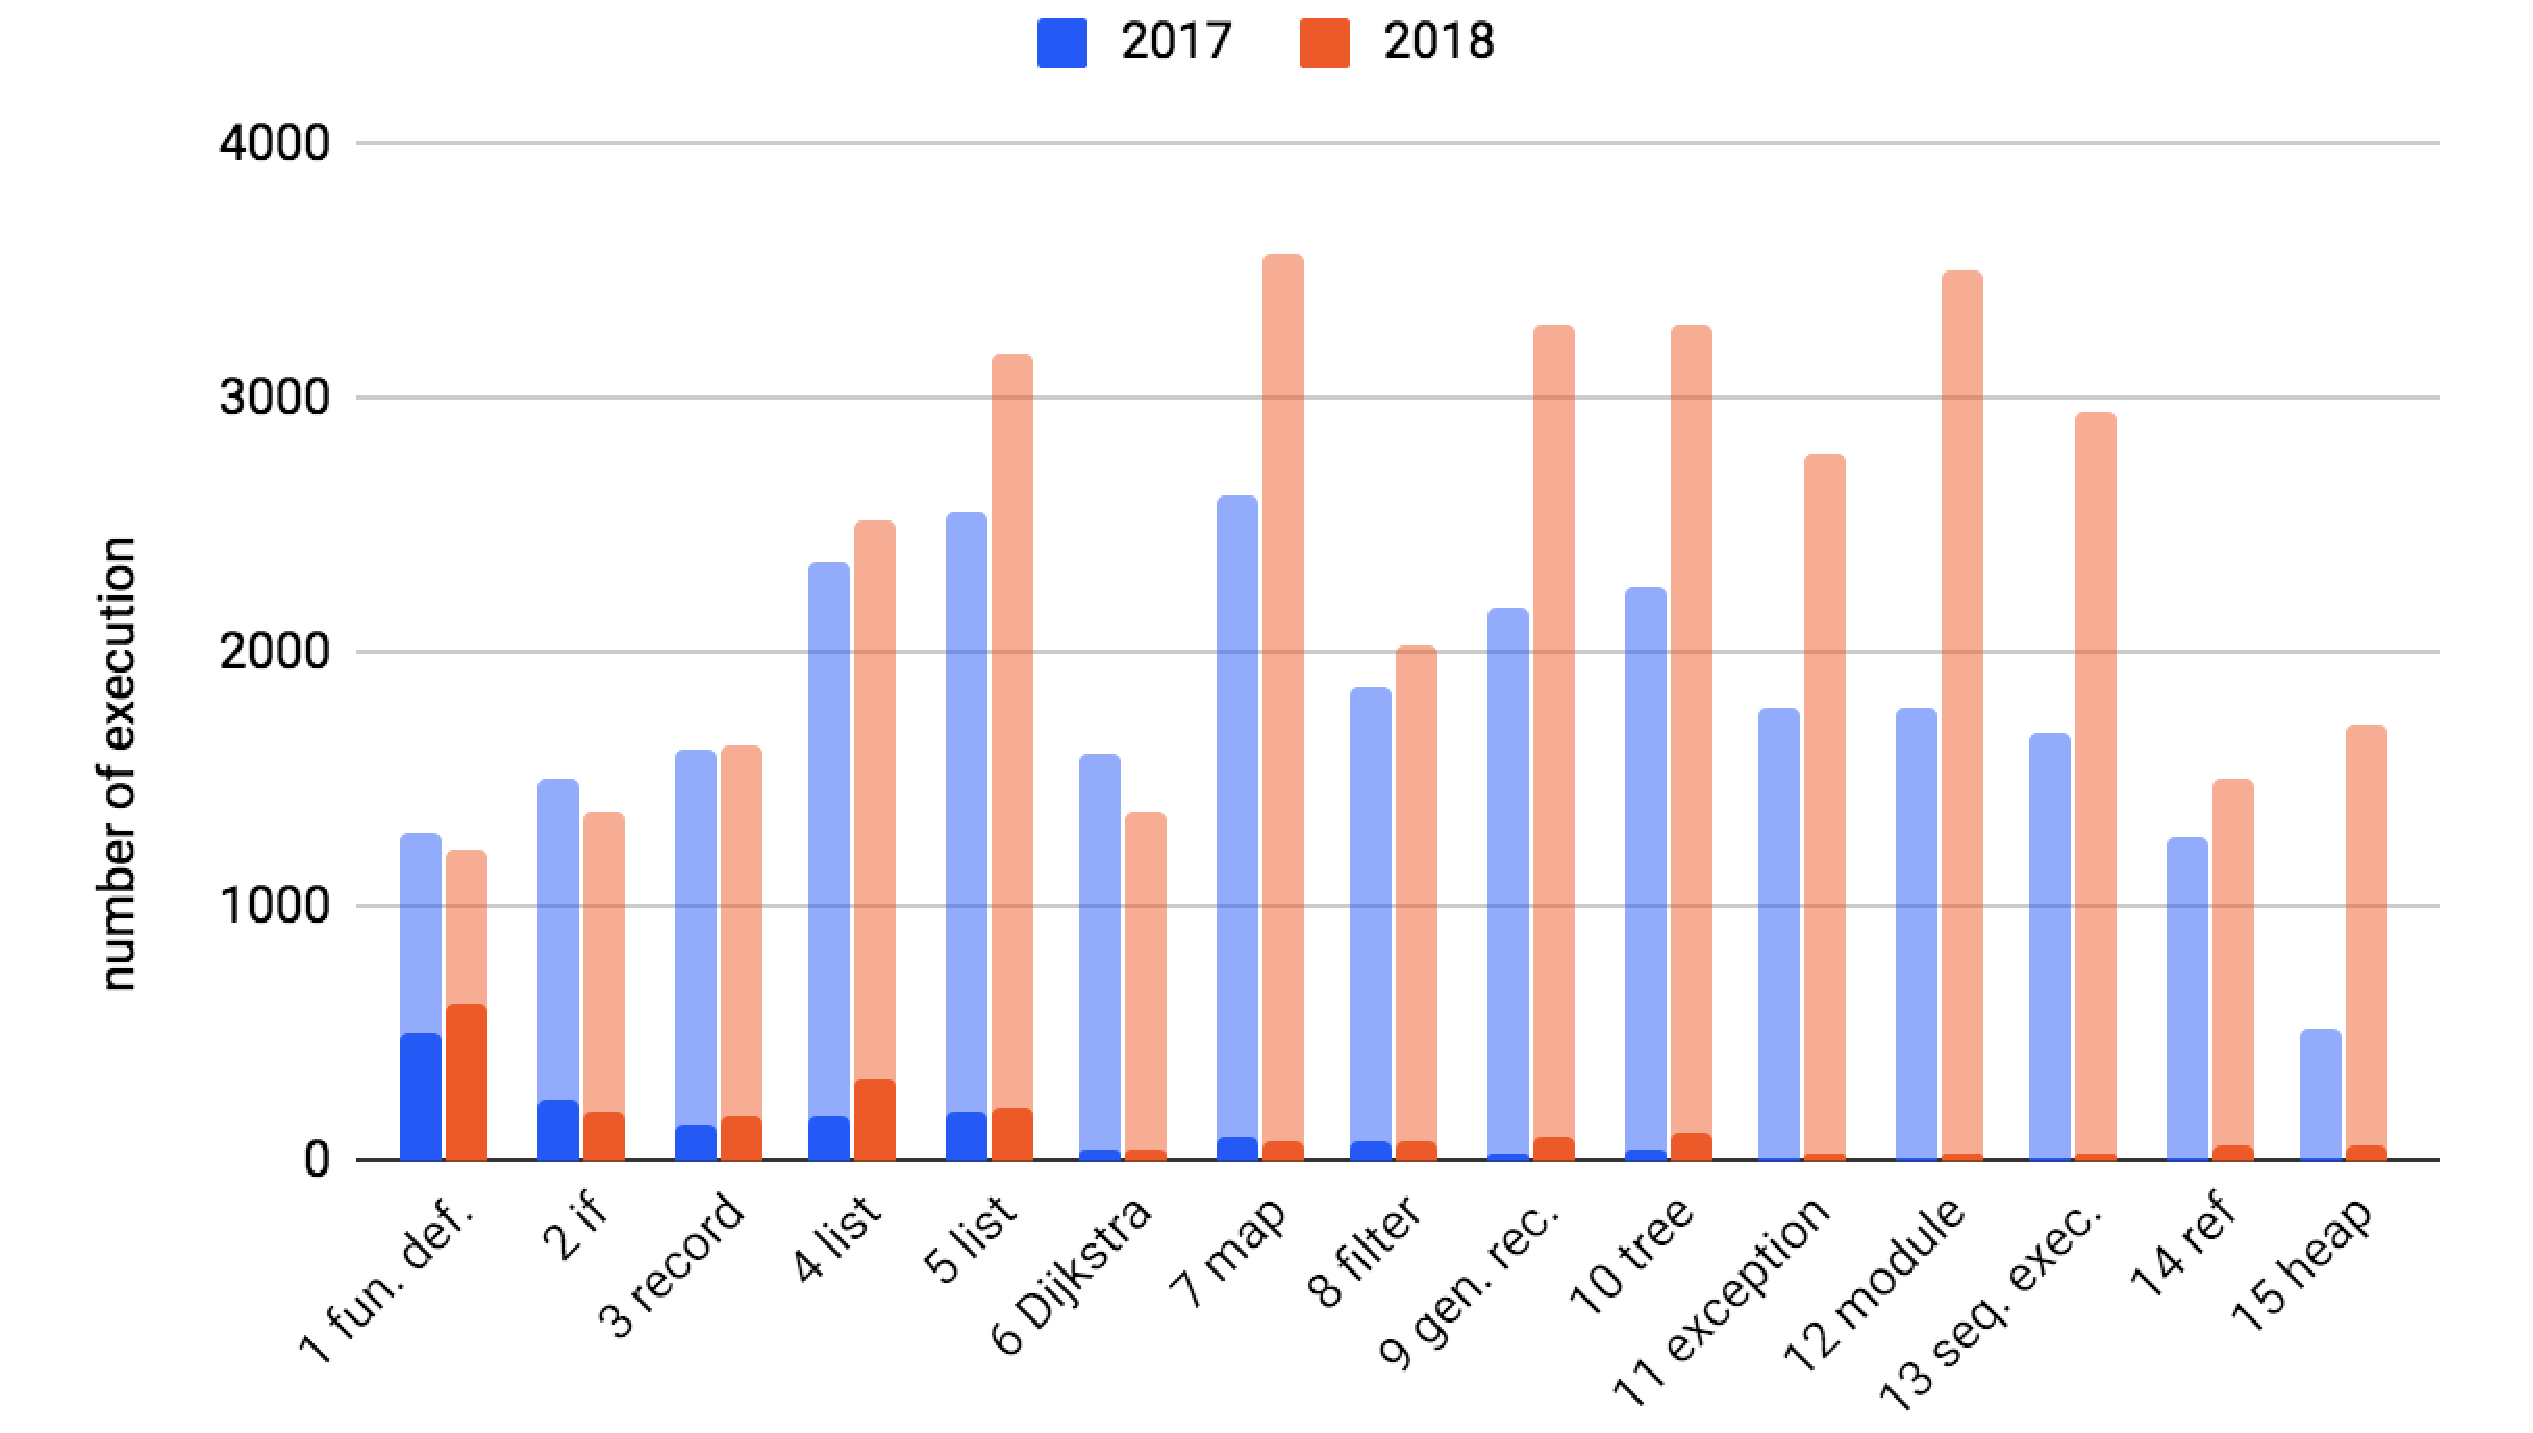
\includegraphics[width=15cm]{6/table1a.eps}
    % \caption{Frequency of standard execution (light-colored) and
    % step execution (dark-colored) in each week in 2017 and 2018.
    % The stepper was not used at all toward the end of the course in 2017,
    % but it was used in some degree in 2018.}
    \caption[ステッパが使用された回数]{
        2017年度と2018年度の各週の、通常の実行 (薄い色) とステップ実行 (濃い色) の回数。
        2017年度は終盤では全く使われなくなったが、2018年度にはある程度使われ続けている。
    }
    \label{figure:allExecution}
  \end{center}
\end{figure}

\begin{figure}[!t]
  \begin{center}
    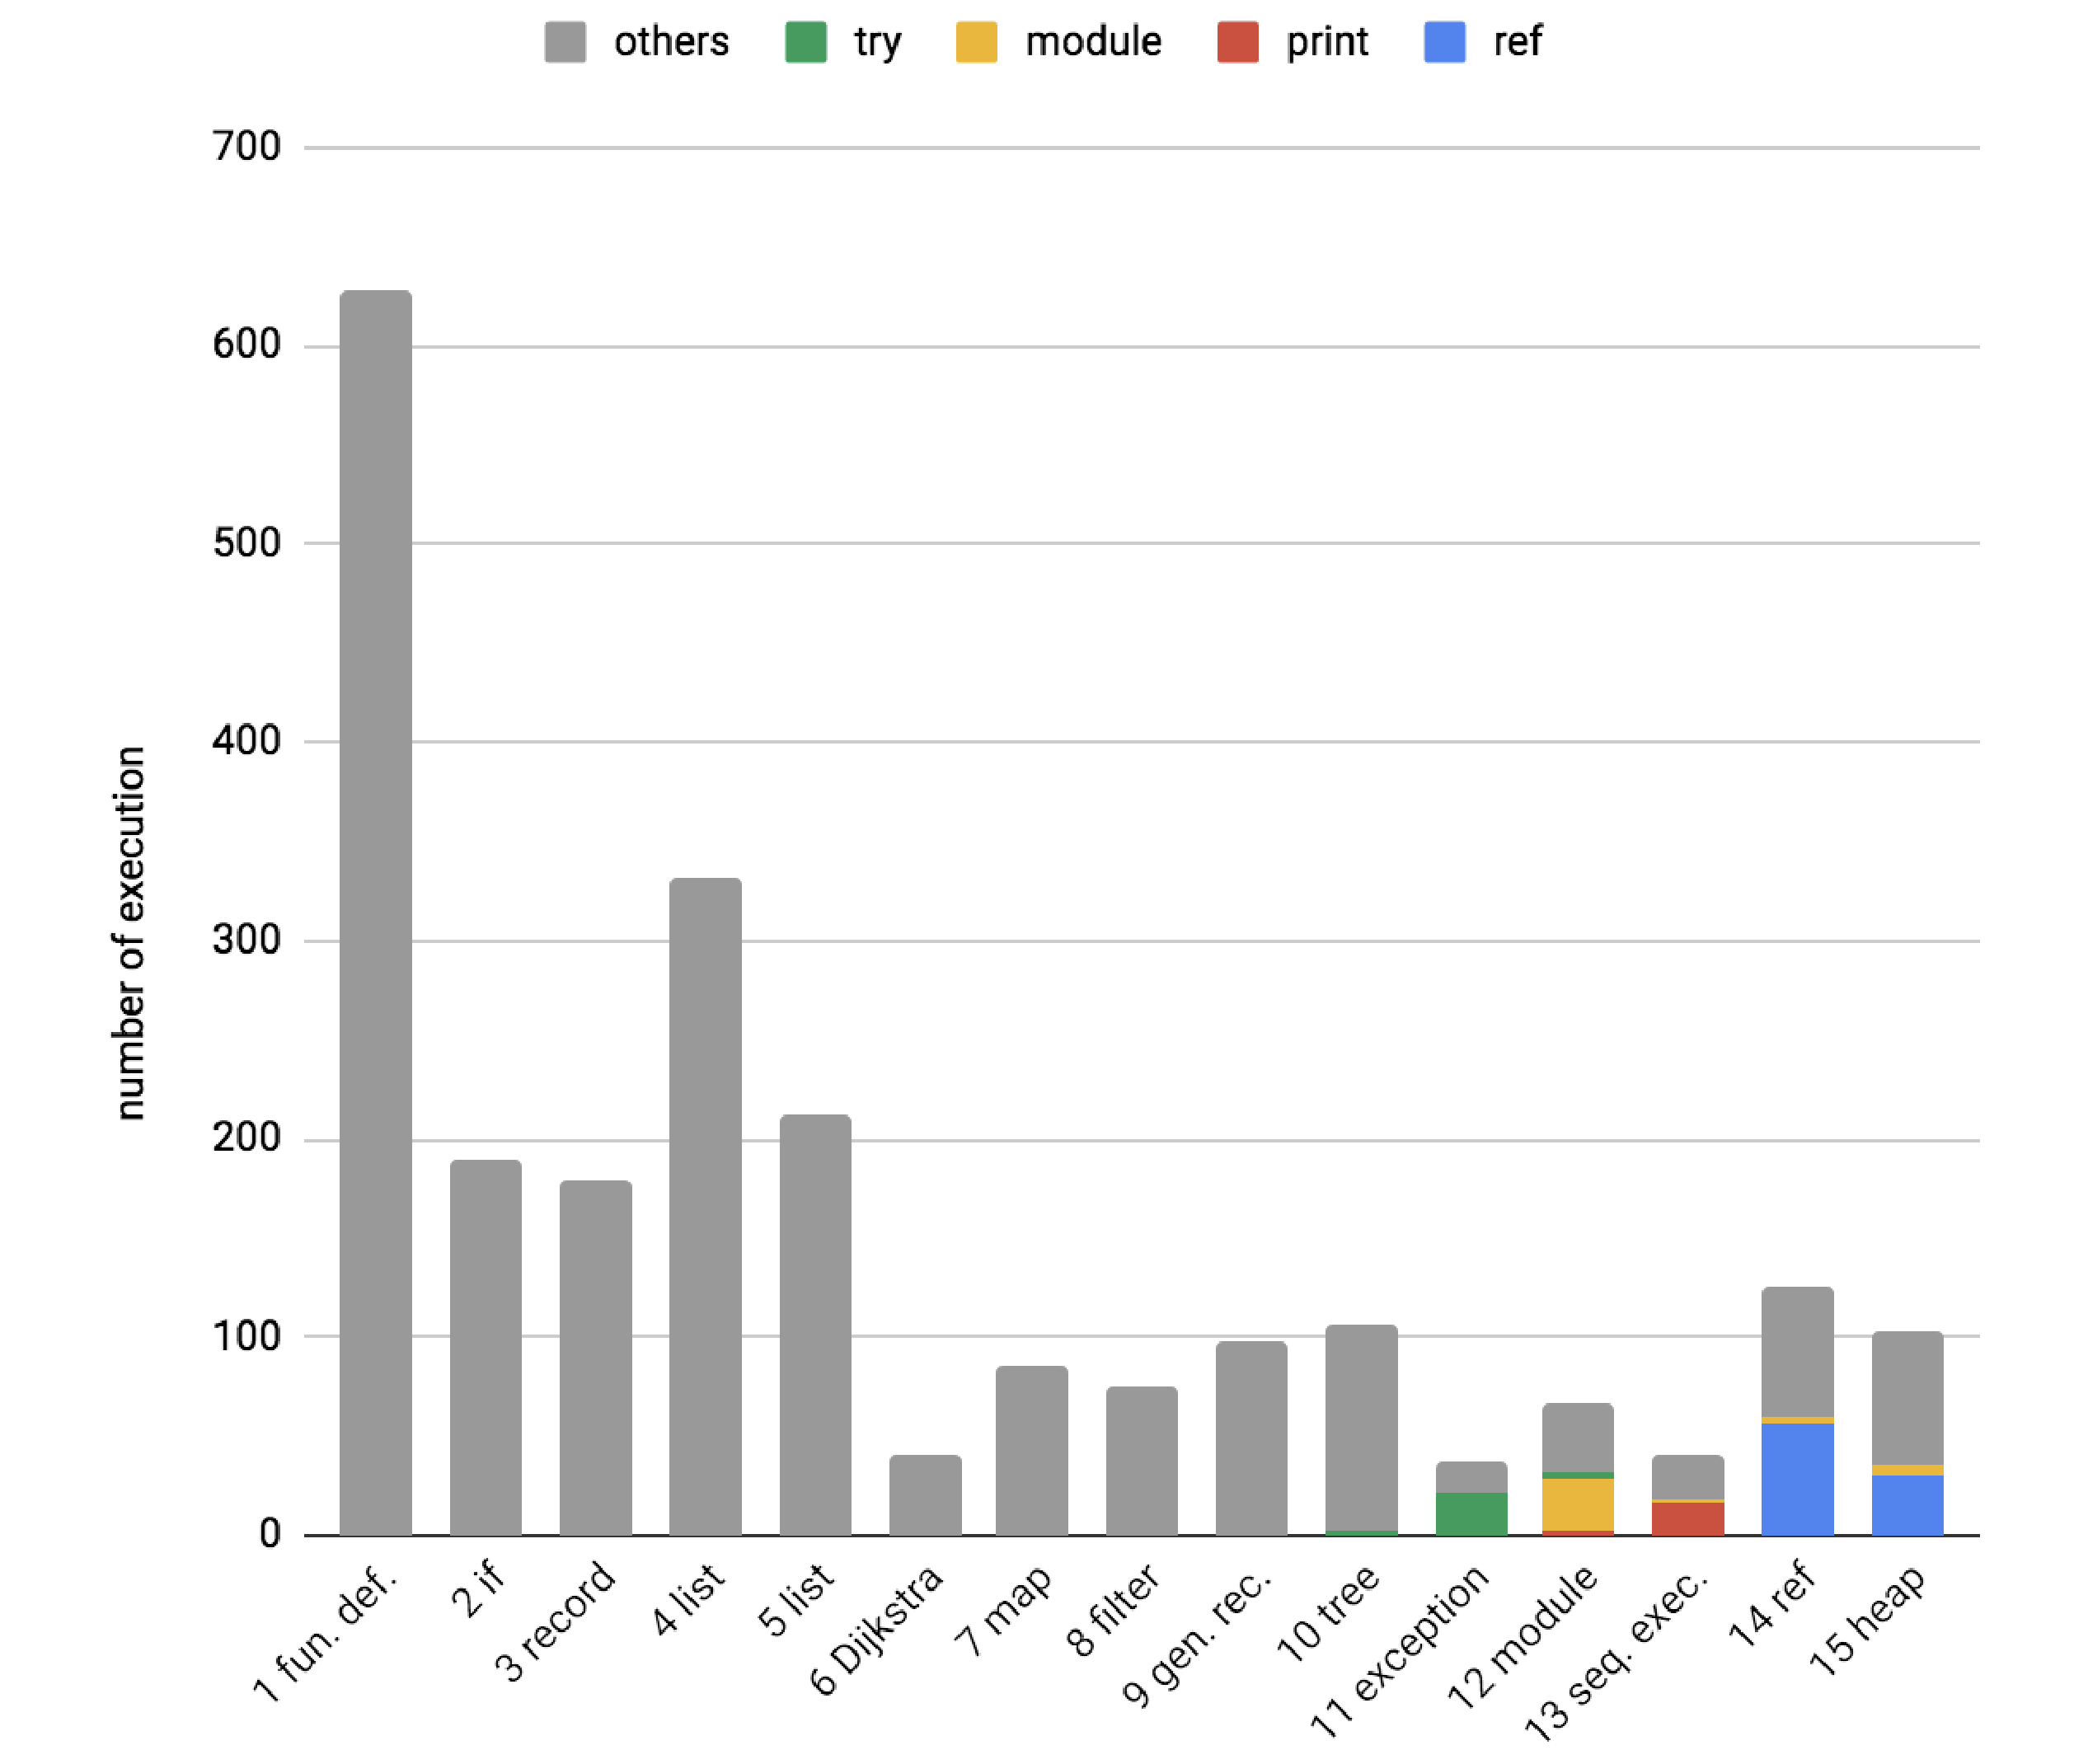
\includegraphics[width=15cm]{6/table1b.eps}
    % \caption{Number of times the stepper was used to evaluate
    % a program with ``try'', ``module'', ``print'' or ``ref'' in 2018.}
    \caption[ステッパの実行のうち各構文を含むプログラムの実行の回数]{
        try、module、print、ref を含むプログラムのステッパによる実行の回数
    }
    \label{figure:stepExecution}
  \end{center}
\end{figure}

% Figure \ref{figure:allExecution} shows
% how many times students used the stepper
% among all the executions including the ones that ended up in an error.
図 \ref{figure:allExecution} は、
全受講生の全実行 (エラー終了した実行を含む) のうち何回がステッパでの実行だったかを示すグラフである。
% In both 2017 and 2018, the stepper was used quite often until week 5.
2017 年度と 2018 年度の両方で、5 週目まではステッパが頻繁に利用されている。
% This is partly because
% we encouraged students to use the stepper when they had
% trouble finding bugs and understanding recursion.
この一因は、バグの発見や再帰の理解のためにステッパを使うように
教員やティーチングアシスタントが学生に勧めたことである。
% After week 5, the number decreases, because students started using an
% interpreter, too, as programs became larger.
6週目以降は、学生がインタプリタに気付き始めたことと
実行するプログラムが大きくなったことにより使用回数が減少した。

% In 2017, the number of stepper uses decreases toward the end of the
% course.
2017 年度には、ステッパの使用回数は最後の授業に近づくにつれて減少している。
% In contrast, in 2018, certain number of stepper uses is observed,
% thanks to the support of exception handling, modules, and references.
それに対して 2018 年度は、例外処理、モジュール、逐次実行、書き換え可能な変数に対応したので、
ある程度の回数の使用が見られる。
% Figure \ref{figure:stepExecution} shows the number of execution of
% programs using these features during step-execution in 2018. % 足した execution を単数にした
図 \ref{figure:stepExecution} は、2018 年度のステップ実行のうち
この年に新しく対応した構文を利用したプログラムの実行の回数のグラフである。
% From the figure, we can see that there is a demand for step
% execution of advanced constructs such as exception handling and
% modules.
どの構文もいくらかステップ実行されており、
例外処理やモジュールのような高度な構文のステップ実行の需要があることが分かる。

% The exact numbers of execution are available in Table \ref{TableUsage} in the Appendix.
図 \ref{figure:allExecution} と図 \ref{figure:stepExecution}
のグラフの正確な数値は付録の表 \ref{TableUsage} に掲載する。

% \subsection{Effects of Stepper}
\subsection{ステッパの効果}
\label{subsection:result__effects}

% It is not easy to see the effect of a tool like a stepper on
% the learning of students.
ステッパのようなツールの教育効果を測ることは簡単ではない。
% In the case of improving error messages of a compiler, for example,
% one can classify various errors and see how many of them are covered
% by the improved error messages objectively.
例えばコンパイラのエラーメッセージ改善の評価ならば、
エラーを分類して改善されたエラーメッセージがそのうちどれほどに対応しているかを見ることができるだろう。
% For the stepper, it is unclear how to show such numeric data.
ステッパにおいては、そういった定量的なデータをどのように示せばよいかが不明瞭である。

\begin{figure}
  \begin{center}
    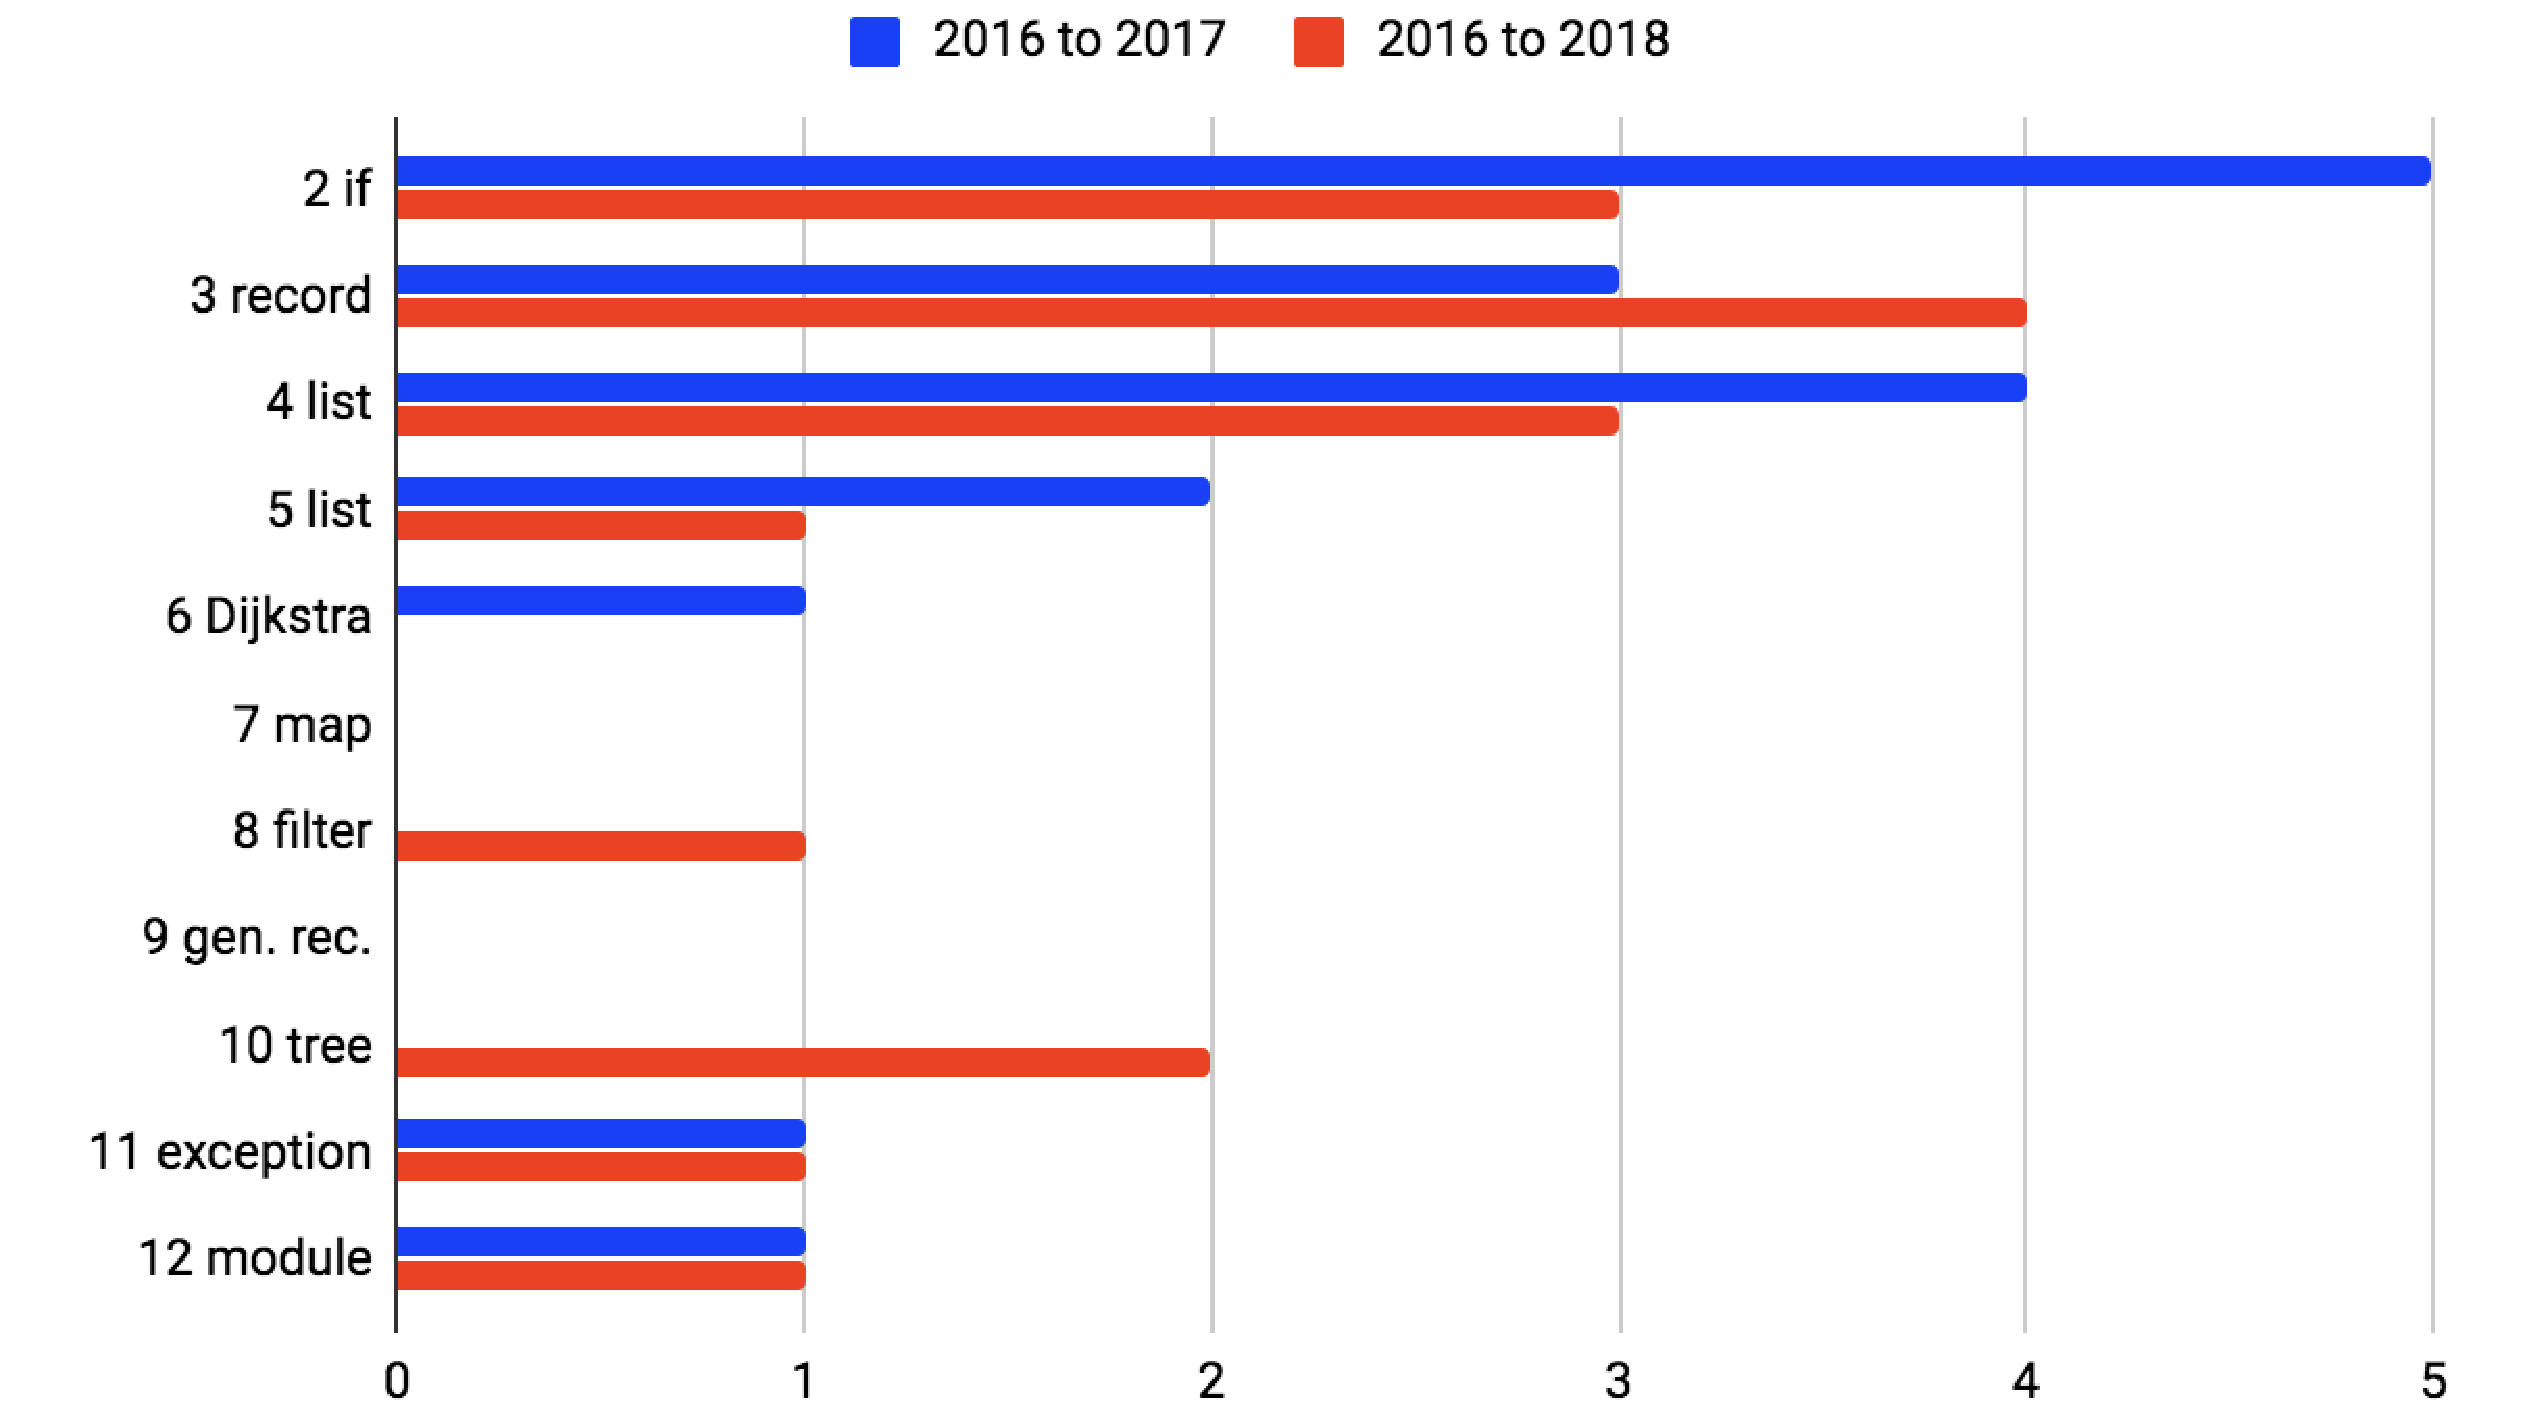
\includegraphics[width=15cm]{6/table2.eps}
    % \caption{Number of questions where students arrived
    % at a correct answer significantly faster in 2017 and 2018 than 2016.}
    \caption[学生が正答するまでの時間の比較]{
        2017年度と2018年度に、学生が2016年度より有意に早く正答を提出した問題の数
    }
    \label{figure:p}
  \end{center}
\end{figure}

% As an attempt to measure the effect of the stepper, we examined how
% long students took to submit correct solutions to the check system.
ステッパの効果を測定するための試みとして、
我々は学生がチェックシステムに正しい解答を提出するまでにかかった時間を調査した。
% Among all the submitted correct solutions, we gathered the (wall-clock) times of
% submissions recorded in the check system that are within 100 minutes
% from the beginning of the class and compared the average times among
% 2016, 2017, and 2018.
全ての問題のチェックシステムに記録されている「正答が初めて提出された時刻」の中から
授業開始から100分以内の時刻を収集し、2016年、2017年、2018年の間で比較した。

% Figure \ref{figure:p} shows the number of questions
% for which students submitted a correct answer
% within significantly shorter time in 2017 and 2018 compared to 2016.
図 \ref{figure:p} は
2017 年度と 2018 年度それぞれの、2016 年度よりも
学生が有意に短い時間で正解を提出した問題の数を示している。
% The data are based on one-sided t-testing with p-value $< 0.05$;
% we refer the reader to Table \ref{TableTTest} of the appendix for details.
このデータは p $< 0.05$ の片側 t 検定に基づいており、
詳しい数値は付録の表 \ref{TableTTest} にある。
% Note that we did not include week 1
% because we had a special pre-test in the first lecture in 2018.
ただし、2018 年度のみ初回の授業に特別なテストを行ったので、
第 1 週はこの調査の対象から外した。

% From the figure, we can see improvement of submission times
% after the (real) introduction of the stepper, especially in earlier problems.
図から、実質的なステッパの導入の後、提出までの時間が改善されていることが分かる。
序盤の問題で特に改善が見られる。
% However, there is an exception: for one problem in the 6th week,
% correct submissions come significantly later in 2018 than in 2016.
しかし 1 つ例外があり、第 6 週の 1 つの問題のみ、
2018 年度の正解提出が有意に 2016 年度よりも遅かった。
% The problem simply asks students
% to write a recursive function that adds 1 to each
% element of a given list.
該当する問題は、リストを受け取ったらそのリストの全要素に 1 を足したリストを返す
再帰関数を書くという単純な問題である。
% We do not know why it took so long in 2018.
この問題の正答が 2018 年度に遅くなった理由は分からない。
% The result of t-testing all the problems together is
% t(1778) = 2.819 (p=0.002) in 2017 and t(2111) = 2.592 (p=0.005) in 2018.
全問題の正答時間をまとめて t 検定した結果は、2017 年度が t(1778) = 2.819 (p=0.002)、
2018 年度が t(2111) = 2.592 (p=0.005) だった。

% We also compared the average times between 2017 and 2018.
2017 年度と 2018 年度の平均時間も比較した。
% For earlier weeks (up to week 5), submissions in 2017 were
% significantly earlier, while for later weeks,
% there were no significant difference
% (except for two problems where the average
% times for 2018 were earlier).
第 5 週までの早い週には 2017 年度の方が有意に早く、
それより後は 2 問のみ 2018 年度の方が早く、あとは有意差は見られなかった。
% Putting all the problems together, the two were not significantly
% different with t(1953)=0.455 (p=0.324).
こちらも全問題の時間をまとめて t 検定すると、t(1953)=0.455 (p=0.324) となり、
有意な差はなかった。

% \paragraph{Threats to validity.}
\paragraph{有効性に対する脅威}
% It is possible that the results of our experiment were affected
% by the enrolled students in each year (there was no over-lapping).
この調査の結果は、各年の学生の影響を受けた可能性がある (同じ学生が 2 度以上履修したことはない)。
% 実験の結果は、毎年入学した学生の影響を受けた可能性があります(重複はありませんでした)。
% In all the three years, 
% the instructor started the class with some introductory comments that
% vary in length.
また、3 年間を通して
毎回の授業時間の最初に教員が前回の課題や今回の内容などについて話す時間をとっており、
その長さは毎回同じではなかった。
% Although the instructor made similar comments in each year, they were
% not exactly the same, which could have affected.
毎年ほとんど同じようなコメントをしてはいるが完全に同じではないので、結果に影響した可能性がある。

% \subsection{Students' Evaluation}
\subsection{学生による評価}
\label{subsection:result__students}

\begin{table}
  \begin{center}
  \begin{tabular}{|l|c|r|}
    \hline
    % & score & \# of students \\ \hline
    & 点数 & 人数 \\ \hline
    % Using the stepper, I could almost always understand & & \\
    % the behavior of programs or the cause of errors. & 4 & 3 \\ \hline
    % Using the stepper, I could often solve problems at hand. & 3 & 8\\ \hline
    % Using the stepper, I could sometimes solve problems at hand. & 2 & 25\\ \hline
    % I could rarely find new things using the stepper. & 1 & 2\\ \hline
    % The stepper was useless.  I did not use the stepper. & 0 & 0\\ \hline
    ステッパを使えばほぼ必ずプログラムの動きや間違いの原因が分かった & 4 & 3\\ \hline
    ステッパを使って問題を解決できることが多くあった & 3 & 8\\ \hline
    たまにステッパを使って問題を解決できることがあった & 2 & 25\\ \hline
    ステッパを使うことで新たに何かが分かることはほとんど無かった & 1 & 2\\ \hline
    全く役に立たなかった、または使わなかった & 0 & 0\\ \hline
%   4 & ステッパを使えばほぼ必ずプログラムの動きや間違いの原因が分かった & 3\\ \hline
%   3 & ステッパを使って問題を解決できることが多くあった & 8\\ \hline
%   2 & たまにステッパを使って問題を解決できることがあった & 25\\ \hline
%   1 & ステッパを使うことで新たに何かが分かることはほとんど無かった & 2\\ \hline
%   0 & 全く役に立たなかった、または使わなかった & 0\\ \hline
  \end{tabular}
  \end{center}
%   \caption{Students' scoring of the stepper in 2018.
%   38 students out of 42 answered.
%   The average is 2.3.}
\caption[学生による点数評価]{2018 年度の学生による点数評価。42 人中 38 人が回答。平均は 2.3 だった。}
% 平均 2.3158、38 / 42 人が回答
  \label{TableScore}
\end{table}

% At the end of the semester of 2018, we asked the students to share
% their thoughts on the stepper.
2018 年度前期の最後に、学生にステッパについてのアンケートを実施した。
% We received responses from 38 out of 42 students.
42 人の受講者のうち 38 人が回答した。
% We first asked whether the stepper was useful on the 0 to 4 point scale.
その中で、ステッパがどれくらい便利だったかを 0 から 4 点で評価してもらった。
% The results, which we present in Table \ref{TableScore}, suggest
% that the stepper is not a silver bullet that is useful
% for all the time.
結果を表 \ref{TableScore} に示す。
この表からはステッパはいつでも役立つ万能なツールではないことが分かる。
% However, most students could solve the problems at hand sometimes
% using the stepper.
しかし、多くの学生がステッパを使って時々問題を解決することができている。
% We are encouraged to see some students choose ``the stepper was almost always useful''.
「ステッパを使えばほぼ必ずプログラムの動きや間違いの原因が分かった」を選んだ学生もいた。

% We next asked students to write when the stepper was useful (if any),
% such as when they found their misunderstanding, or when they could
% deepen their understanding.
他の質問で、
プログラムの間違いの発見や理解のためにステッパを活用できた場面を (あれば) 答えてもらった。
% We summarize the answers in two categories.
その答えを 2 つに分類して紹介する。

% \paragraph{Understanding of the behavior of programs.}
\paragraph{プログラムの挙動の理解}
% Seven students answered they could deepen their understanding of
% the behavior of programs.
7 人の学生が、プログラムの挙動についての理解を深めることができたと答えた。
% In particular, five students among them wrote explicitly that the
% stepper helped them figure out how functions consume recursive data.
特にその内 5 人が関数がどのように再帰的なデータを消費するのかを把握するのに役立ったと書いている。
% 特に、そのうち5人の学生は、関数が再帰データをどのように消費するかを把握するのにステッパーが役立つと明示的に書いています。
% We imagine it was particularly instructive to see how a recursive 
% function definition is unfolded in nesting application.
再帰関数定義が展開されて関数適用の入れ子になっていく様子を見ることができることは
再帰の理解の助けになると考えられる。

% Other students answered that they could observe the behavior of
% programs in general.
他の学生は、プログラム全般の動きを観察できたと答えた。
% They found that arguments of a function are evaluated before the
% function call, and that the elements of a list are evaluated one by one.
その学生たちは、引数が関数呼び出しの前に 1 つずつ実行されることを発見した。
% Among them, one student observed the right-to-left execution
% employed in OCaml.
1 人は OCaml プログラムが right-to-left で実行されていることに気付いた。
% Previously, such subtle behavior was taught only in passing without
% much emphasis.
以前は、このような細かい動作について特に強調せず授業を進めていた。

% \paragraph{Debugging.}
\paragraph{デバッグ}
% Many students found the stepper useful for debugging.
多くの学生がデバッグにステッパを利用できたと回答した。
% Sixteen students answered they could find what was wrong when their
% program did not pass test cases.
16 人の学生が、テストを通らなかった時にどこが間違っているのかを見つけることができたと回答した。
% By observing each step of execution, they could identify when the
% program behaved differently from their expectation.
実行の各ステップを観察することで、期待と違った振る舞いをする箇所を特定することができたという。
% This is an important step toward debugging in general.
これは一般的なデバッグをする上で重要な過程である。
% Because printing (and side effects) is handled at the end of the
% course, the only debugging method for students had been unit testing:
% they checked whether all the component functions worked as expected.
この授業では出力などの副作用を終盤で学習するので、
学生のデバッグの方法は単体テストで関数全体が正しい値を返すかどうかを見るしかなかった。
% With the stepper, they can simply observe execution of the program and
% see when it goes wrong.
しかしステッパがあれば、
学生は実行中のどこで間違いが起きているのかを単純に観察することができる。

% Three students found the stepper useful to understand why their
% program did not terminate.
% Without printing, it is not easy for students to identify the cause of
% infinite loops.
また、3 人の学生がプログラムが停止しない時にその原因をステッパで突き止めることができた。
出力機能を使わずに無限ループの原因を特定することにもステッパは利用できる。
% Using the stepper, one of the students could not only observe
% the infinite loop, but also see how far her progr went well
% and when it went wrong.
% ここは書かない・・・



\newpage
\chapter*{謝辞}

・浅井先生
・叢さん
・石尾氏
・北川氏
・1学年上の研究室の人
・家族
・祖父母
・PPL 2018 と PPL 2019 でなにか言ってくれた人々
・戸次先生
・ステッパを使わされた学生
・株式会社 HERP の人々
〜に感謝いたします.


\newpage
%参考文献をしめします.


\begin{thebibliography}{3}
\bibitem {bunken} 参考文献は,本または論文のタイトル,著者名,出版社,ページ(論文の場合),発行年を記すこと.
\bibitem{latex2e}
乙部巌己,江口庄英,
pLaTeX2ε for Windos,SOFT BANK,1996.
\end{thebibliography}


\newpage

%付録
\appendix
\chapter{実験でもちいたデータ}

ここには,実験のデータなど,論文の本文中に載せられなかったが,
読者にとって役に立つとおもわれるデータなどを付録として掲載する.

\chapter{ふろく}

\section{section}

\section{2}

\chapter{furoku}


\end{document}
